%&../../.preamble
\endofdump
\usepackage{layouts}
\usepackage{tabularx}
\usepackage{makecell}\usetikzlibrary{patterns}
\usepackage{contour}

\usepackage{pgf-umlcd}

\makeatletter
\newcommand\HREF[2]{\hyper@linkurl{#2}{#1}}
\makeatother

\title{Ripetizioni informatica}
\author{Mattia Marini}
\date{Agosto 2023/2024}
\begin{document}
\maketitle
\license{Ripetizioni informatica}
\tableofcontents
\listofexercises

\newpage
% A grandi linee vedremo:
% \begin{itemize}
% 	\item Da c++ a java
% 	      \begin{itemize}
% 		      \item Aspetti comuni
% 		            \begin{itemize}
% 			            \item Istruzioni e commenti
% 			            \item Definizione funzioni e variabili
% 			            \item Strutture di controllo (\verb|for| e \verb|while|)
% 		            \end{itemize}
% 		      \item Differenze
% 		      \item Object orientation
% 		      \item Uso della memoria (no puntatori \textit{gabare collection})
% 	      \end{itemize}
% 	\item Introduzione programmazione ad oggetti
% 	      \begin{itemize}
% 		      \item Classi e oggetti
% 		      \item Attributi e metodi
% 		      \item Oggetti vs tipi primitivi
% 	      \end{itemize}
% 	\item Definizione di classi
% 	      \begin{itemize}
% 		      \item Costruttori
% 		      \item Visibilità metodi
% 		      \item Getters and setters (\textit{encapsulation}, \textit{information hiding})
% 		      \item Metodi/variabili statiche
% 	      \end{itemize}
% 	\item Ereditarietà e polimorfismo
% 	      \begin{itemize}
% 		      \item Utilizzo e potenzialità a livello intuitivo
% 		      \item Estendere classi (\textit{ereditarietà singola})
% 		            \begin{itemize}
% 			            \item Costruttore (keyword \verb|super|)
% 			            \item Aggiunta metodi
% 			            \item Overriding e overloading
% 		            \end{itemize}
% 		      \item Di nuovo modificatori visibilità (\verb|public private protected package|)
% 		      \item Concetto formale di \underline{dinamic binding}, tipo statico e tipo dinamico
% 		      \item Classi e metodi astratti
% 		      \item Interfacce (\textit{soluzione a polimorfismo parametrico})
% 	      \end{itemize}
% \end{itemize}
\newpage
\renewcommand{\arraystretch}{1.5}
\section{Da c++ a java}
Java è molto simile dal punto di vista della sintassi al c++. Non sarà molto complicato il passaggio
\subsection{Aspetti simili}
La sinttassi di Java è molto simile a quella di c++, ecco gli aspetti che rimangono invariati o quasi:
\subsubsection{Dichiarazione delle variabili:}
\begin{center}
	\begin{tabularx}{\linewidth}{lX}
		\toprule
		Sinstassi                          & Differenze rispetto al \verb|c++|                                                                              \\
		\midrule
		\verb|int x = 15|                  & invariato                                                                                                      \\

		\verb|long x = 15|                 & invariato                                                                                                      \\

		\verb|float x = 15.0f|             & nota il \verb|15.0f|, dove \verb|f| sta per float                                                              \\

		\verb|double x = 15.0|             & float ma con precision maggiore, 64 bit                                                                        \\

		\verb|boolean x = true|            & \verb|boolean| anzichè \verb|bool|                                                                             \\

		\verb|String s = "stringa"|        & dato \verb|String| sarebbe una classe ma è trattato come tipo primitivo, dato che è usato molto frequentemente \\

		\verb|String v[] = new String[15]| & vettore di stringhe di dimensione 15                                                                           \\

		\verb|int v[] = new int[15]|       & vettore di interi di dimensione 15                                                                             \\
		\bottomrule
	\end{tabularx}
\end{center}
\subsubsection{ Commenti:}
\begin{itemize}
	\item Commento riga singola: \verb|// commento|
	\item Commento righe multiple: \verb|/* commento */|
\end{itemize}
\subsubsection{ Cicli:}
\begin{itemize}
	\item Ciclo for:
	      \begin{lstlisting}[language = c, frame = none, numbers = none]
          for(int i = 0; i<15; i++){
            // qualcosa
          }
        \end{lstlisting}
	\item Ciclo while:
	      \begin{lstlisting}[language = c, frame = none, numbers = none]
          while(i < 15){
            // qualcosa
          }
        \end{lstlisting}
\end{itemize}
\subsubsection{Operatori}
\begin{center}
	\begin{tabular}{l  l}
		\toprule
		\sfblue{Operatore}                     & \sfblue{Descrizione} \\
		\midrule
		{ \ttfamily + \quad - \quad * \quad /} & operatori matematici \\
		{ \ttfamily \&\& }                     & and logico           \\
		{\ttfamily $ || $}                     & or logico            \\
		{\ttfamily $ ! $ }                     & not logico           \\
		\bottomrule
	\end{tabular}
\end{center}
\subsubsection{If e switch}

\begin{minipage}[t]{0.48\linewidth}
	\begin{lstlisting}[language = c, frame = none]
  if(a<b) {
    //codice
  }
  else(if a>b) {
    //codice
  }
  else {
    //codice
  }
        \end{lstlisting}
\end{minipage}
%
\begin{minipage}[t]{0.48\linewidth}
	\begin{lstlisting}[language = c, frame = none]
switch(espressione) {
  case x:
    // codice
    break;
  case y:
    // codice
    break;
  default:
    // codice
}
        \end{lstlisting}
\end{minipage}
\subsubsection{Funzioni}
\begin{lstlisting}[language = c, frame = none]
  void nome_funzione1 (int arg_1, String arg_2){
    //corpo funzione
  }

  int nome_funzione2 (int arg_1, String arg_2){
    //corpo funzione
    return 5;
  }
        \end{lstlisting}

Una funzione è quindi definita indicando nel seguente ordine, esattamente come in c++:
\begin{enumerate}
	\item \underline{Tipo di ritorno} (o \verb|void| se non ritorna nulla)
	\item \underline{Nome} della funzione
	\item \underline{Parametri}, racchiusi fra parentesi tonde e separati da virgole
	\item \underline{Corpo} della funzione fra graffe
\end{enumerate}
\subsection{Differenze}
\subsubsection{Stampa su terminale}
Una delle feature usata moltissimo, ma completamente diversa dal c++ è la stampa su terminale:
\begin{lstlisting}[frame = none]
  System.out.println("Stampa questa cosa");
  //stampa andando a capo prima di stampare

  System.out.print("Stampa questa cosa");
  //stampa SENZA andando a capo
\end{lstlisting}

\vskip3mm
nota che le stringhe si possono concatenare con l'operatore +:

\vskip3mm
\begin{lstlisting}[frame = none]
  String a = "Hello";
  String b = "world";

  System.out.println(a + b);
  //stampa "Hello world"

  String c = a + b;
  //Inizializza c a "Hello world"
  
\end{lstlisting}
\subsubsection{Linguaggio interpretato vs compilato}
A differenza di c++, java è un linguaggia \underline{interpretato}
\begin{itemize}
	\item \textit{Linguaggio compilato}: il codice è "dato in pasto" a un compilatore, il quale lo converte in linguaggio macchina (di fatto in una sequenza di, 0 ed 1)
	\item \textit{Linguaggio interpretato}: il codice è "dato in pasto" ad un compilatore, il quale lo converte però in \underline{bytecode}, ossia un linguaggio di basso livello (molto difficile da leggere e scrivere), il quale è in grado di essere letto da un \textit{interprete}
\end{itemize}

\begin{center}
	\begin{tabular}{c c}
		\begin{forest}
			for tree={draw, grow = -90}
			[codice c++ [compilatore c++ , draw = none [assembly [assemblatore, draw = none [linguaggio macchina [computer, circle]]]]]]
		\end{forest}
		 &
		\begin{forest}
			for tree={draw, grow = -90}
			[codice java [compilatore java , draw = none [java bytecode [java interpreter [computer, circle]]]]]
		\end{forest}
	\end{tabular}
\end{center}
\subsubsection{Memoria e puntatori}
Java è un linguaggio ad alto livello che gestisce la memoria in maniera diversa rispetto al c++:
\begin{itemize}
	\item c++: il compito di allocare e deallocare la memoria non più utilizzata è del programmatore
	\item java: la memoria viene deallocata in maniera automatica tramite un meccanismo chiamato \underline{garbage collection}
\end{itemize}

Visto che in java la memoria è gestita in in maniera automatica, il programmatore non ne ha accesso diretto tramite puntatori: al contratio, i puntatori \underline{non esistono}

\subsubsection{Object orientation}
Sebbene c++ sia un linguagio che permette di utilizzare classi ed oggetti, in java l'object orientation è forzata: ogni parte del programma deve essere contenuta all'interno di una classe

\subsection{Esempio programma}
\begin{lstlisting}[language = c++, frame = none]
class HelloWorld {
    public static void main(String[] args) {
        System.out.println("Hello, World!"); 
    }
}
\end{lstlisting}

Cose da notare:
\begin{itemize}
	\item La funzione main è contenuta all'interno di una classe "HelloWorld", il cui nome è arbitrario
	\item La funzione main è marcata come \verb|static|, ciò vuol dire che la funzione esiste anche se non esiste un oggetto di tipo "HelloWorld", affroteremo meglio il modificatore \verb|static| più avanti (sez. \ref{static}), per ora possiamo ignorarlo
	\item La funzione main è marcata come \verb|public|, ciò vuol dire che la funzione è accessibile ovunque. Afffronteremo meglio questo modificatore più avanti, per ora possiamo ignorarlo
	\item La funzione main prende in ingresso un vettore di stringhe. Nel caso si avviasse l'applicazione da terminale e possibile passare al main dei parametri nel seguente modo:
	      \begin{lstlisting}[language = bash, frame = none]
  cd cartella_applicazione 
  ./nome_applicazione parametro_1 parametro_2 ... \end{lstlisting}
	      in questo caso il vettore di stringhe \verb|args| conterrà \verb|parametro_1| e \verb|parametro_2|. Penso non lo userete mai ma è buono saperlo
\end{itemize}
\subsection{Funzioni utili}
In java sono definite alcune funzioni utilissime. Qui una lista (non esaustiva) delle più comuni:
\subsubsection{Stringhe}

Supponiamo di avere \verb|String s = "stringa stringa";|
\vskip3mm
\begin{tabularx}{\linewidth}{lX}
	\toprule
	\sfblue{Funzione}                & \sfblue{Descrizione}                                                                  \\
	\midrule
	\verb|s.lenght()|                & Ritorna il numero di caratteri conenuti nella stringa (7 nel caso d'esempio)          \\
	\verb|s.charAt(int index)|       & Ritorna il carattere in posizione \verb|index|                                        \\
	\verb|s.indexOf(char carattere)| & Ritorna l'indice della prima occorrenza di \verb|carattere| in \verb|s|               \\
	\verb|s.indexOf(String stringa)| & Ritorna l'indice della prima occorrenza della sottostringa \verb|stringa| in \verb|s| \\
	\bottomrule
\end{tabularx}

\vskip3mm
\begin{lstlisting}[language = c++, frame = none]
    String s = "stringa stringa";
    s.lenght(); // 15
    s.charAt(2); // 'r'
    s.indexOf('r'); // 2
    s.indexOf("ga"); // 5 \end{lstlisting}
\subsubsection{Vettori}
Supponiamo di avere \verb|int v[] = new int[15];|
\begin{center}
	\begin{tabularx}{\linewidth}{lX}
		\toprule
		\sfblue{Funzione} & \sfblue{Descrizione}                               \\
		\midrule
		\verb| v.lenght|  & ritorna il numero di elemnti contenuti nel vettore \\
		\bottomrule
	\end{tabularx}
\end{center}
\subsubsection{Altre funzioni utili}
\begin{center}
	\begin{tabularx}{\linewidth}{lX}
		\toprule
		\sfblue{Funzione}                 & \sfblue{Descrizione}                                  \\
		\midrule
		\verb|Math.exp(float n)|          & Ritorna $ e^n $                                       \\
		\verb|Math.log(float n)|          & Ritorna $ ln\left(n\right) $                          \\
		\verb|Math.abs(float x)|          & Ritorna $ \left|x\right| $ (valore assoluto di $ x $) \\
		\midrule
		\verb|Math.sin(float x)|          & Ritorna $ \sin \left(x\right) $                       \\
		\verb|Math.cos(float x)|          & Ritorna $ \cos \left(x\right) $                       \\
		\verb|Math.tan(float x)|          & Ritorna $ \tan  \left(x\right) $                      \\
		\verb|Math.asin(float x)|         & Ritorna $ \arcsin \left(x\right) $                    \\
		\verb|Math.acos(float x)|         & Ritorna $ \arccos \left(x\right) $                    \\
		\verb|Math.atan(float x)|         & Ritorna $ \arctan  \left(x\right) $                   \\
		\midrule
		\verb|Math.max(float a, float b)| & Ritorna l'elemento maggiore fra $ a $ e $ b $         \\
		\verb|Math.min(float a, float b)| & Ritorna l'elemento maggiore fra $ a $ e $ b $         \\
		\midrule
		\verb|Math.floor(float x)|        & Arrotonda per difetto $ x $                           \\
		\verb|Math.ceil(float x)|         & Arrotonda per eccesso $ x $                           \\
		\verb|Math.round(float x)|        & Arrotonda $ x $                                       \\
		\bottomrule
	\end{tabularx}
\end{center}

\addtocontents{exe}{\protect{\large \vskip3mm \textit{Esercizi introduttivi}\vskip3mm}}
\subsection{Esercizi}
\begin{esercizio}{Somma float}
	Scrivi un programma che dichiari 3 float con valore 15, 12.5 e -12 e ne stampi la somma
\end{esercizio}
\begin{esercizio}{Concat stringhe}
	Scrivi un programma che date due stringhe contenenti nome e cognome, stampi l'uno concatenao all'altro, separati da uno spazio
\end{esercizio}
\begin{esercizio}{Incrementa vettore}
	Scrivi un programma che dato un vettore di interi, incrementi di 1 ogni suo elemento
\end{esercizio}
\begin{esercizio}{Funzione 1}
	Ripetere l'esercizio precedente, spostando il codice all'interno di una funzione apposita
\end{esercizio}
\begin{esercizio}{Funzione stampa pari}
	Creare una funzione che prenda in input un vettore di interi e ne stampi solo gli elementi pari
\end{esercizio}
\begin{esercizio}{Smista stringhe}
	Creare una funzione che prenda in input un vettore di stringhe e un intero $ n $. Ritornare un vettore contenente solo le stringhe con lunghezza minore o uguale $ n $
\end{esercizio}

\section{Classi e oggetti}
Immaginiamo di voler rappresentare un dato "custom", che non è presente di default in java. Supponiamo di dover rappresentare un punto su un piano cartesiano. Questo dato deve:
\begin{itemize}
	\item Contenere informazioni riguardo la posizione ($ x $ e $ y $)
	\item Permetterci di stamparlo a terminale
	\item Permetterci di calcolarne la distanza dall'origine e da un altro punto
\end{itemize}
In questo caso le classi permettono di fare esattamente ciò che vogliamo: \textit{creare un nuovo tipo di dato che possa contenere dei valori e supportare determinati tipi di funzioni}

\begin{tcolorbox}
	Una \underline{classe} non è altro che un insieme di variabili, dette \underline{attributi}, e di funzioni che possono agire su di esse, dette \underline{metodi})
\end{tcolorbox}

La \underline{classe} va a definire "lo scheletro" del dato che vogliamo creare. In poche parole andiamo a elencare quali dati contiene e quali funzioni supporta. Ad esempio, per definire una classe con le funzionalità elencate pocanzi potremmo scrivere il seguente codice:
\vskip3mm
\begin{lstlisting}[language = c++, frame = none]
class Coordinata {

  double x = 10.0; //attributo
  double y = 12.5; //attributo

  // metodo
  public void stampa() {
    System.out.println("(" + x + ", " + y + ")");
  }

  // metodo
  public double distanzaOrigine() {
    return Math.sqrt(x * x + y * y);
  }

  // metodo
  public double distanzaCoordinata(coordinata c) {
    double deltaX = c.x - x;
    double deltaY = c.y - y;
    return Math.sqrt(deltaX * deltaX + deltaY * deltaY);
  }

}
\end{lstlisting}
\vskip3mm
Per utilizzare questo dato, possiamo scrivere:
\begin{center}
	\verb|Coorinata nomeCoordinata = new Coordinata();|
\end{center}
La variabile "nomeCoordinata" è detta \underline{oggetto} o \underline{istanza} di tipo \verb|Coordinata|. Posso ora riferirmi agli attributi e metodi che ho definito prima nel seguente modo:
\begin{lstlisting}[language = c++, frame = none]
nomeCoordinata.x;
nomeCoordinata.y;

nomeCoordinata.stampa();
nomeCoordinata.distanaOrigine();
nomeCoordinata.distanzaCoordinata(new Coordinata())
\end{lstlisting}
\vskip3mm
Nota che:
\begin{itemize}
	\item Il nome della classe "Coordinata" è scritto con la lettera maiuscola. Questa è una \textit{convenzione} importante: il programma funzionerebbe anche se non mettessimo la maiuscola, però per questioni di leggibilità del codice si è deciso che il nome delle classi va sempre con la maiuscola
	\item La classe va dichiarata all'esterno della classe main. Se usate Eclipse o Intellij ogni classe è bene che venga dichiarata come \verb|public class NomeClasse{}| in un file separato, con nome "NomeClasse.java"
	\item Le funzioni sono marcate come \verb|public|. Questo significa che possono essere chiamate in qualsiasi punto del programma. Vedi sezione \ref{modificatoriVisibilità}
\end{itemize}
\subsection{Costruttore}
Quando creiamo un oggetto è utile avere un modo per inizializzare i suoi attributi. Il \underline{costruttore} di una classe è una funzione specializzata, definita all'interno della classe che fa proprio questo.
\begin{itemize}
	\item Il costruttore è una funzione \verb|public| che ha \underline{lo stesso nome della classe}
	\item Il costruttore viene invocato implicitamente quando creiamo un oggetto
	\item Il costruttore \underline{non} ha un valore di ritorno
\end{itemize}
Riprendendo l'esempio di prima, possiamo implementare un costruttore come segue:
\vskip3mm
\begin{lstlisting}[language = c++, frame = none]
class Coordinata {

  double x; // attributo
  double y; // attributo

  //costruttore
  public Coordinata(double newX, double newY) {
    x = newX;
    y = newY;
  }

  // metodo
  public void stampa() {
    System.out.println("(" + x + ", " + y + ")");
  }

  // metodo
  public double distanzaOrigine() {
    return Math.sqrt(x * x + y * y);
  }

  // metodo
  public double distanzaCoordinata(coordinata c) {
    double deltaX = c.x - x;
    double deltaY = c.y - y;
    return Math.sqrt(deltaX * deltaX + deltaY * deltaY);
  }

}
\end{lstlisting}

Ora possiamo (e dobbiamo) creare oggetti scrivendo
\begin{center}
	\verb|Coorinata nomeCoordinata = new Coordinata(15.0, 12.5);|
\end{center}
dunque con la keyword \verb|new| viene invocato implicitamente il costruttore della classe, che ne inizializza gli attributi $ x $ e $ y $

\subsubsection{La keyword "this"}
Quando definiamo un costruttore può essere intuitivo dare ai parametri della funzione lo stesso nome dei corrispettivi attributi, tuttavia così facendo si creerebbe anbiguità:

\begin{lstlisting}[language = c++, frame = none]
class Coordinata {

  double x; // attributo
  double y; // attributo

  //costruttore
  public Coordinata(double x, double y) {
    x = x; //a quale x mi sto riferendo?
    y = y; //a quale y mi sto riferendo?
  }
  //...
}
\end{lstlisting}

in questo caso torna utile una keyword specifica: \verb|this|. \verb|this| all'interno di un classe non è altro che un riferimento alla istanza della classe stessa. Posso quindi riscrivere il costruttore così:
\vskip3mm
\begin{lstlisting}[language = c++, frame = none]
class Coordinata {

  double x; // attributo
  double y; // attributo

  //costruttore
  public Coordinata(double x, double y) {
    this.x = x; //this.x si riferisce all'attributo x, mentre x al parametro del costruttore
    this.y = y; //this.y si riferisce all'attributo y, mentre x al parametro del costruttore
  }
  //...
}
\end{lstlisting}

\subsection{Modificatori visibilità}\label{modificatoriVisibilità}
Abbiamo visto che prima del metodi si può usare la parola \verb|public|. Questo è un \underline{modificatore di visibilità} e serve a specificare da quale parte del codice è possibile invocare il metodo. I modificatori possono essere applicati anche agli attributi. I modificatori sono i seguenti:

\begin{center}
	\begin{tabularx}{\linewidth}{lX}
		\toprule
		\sfblue{Modificatore} & \sfblue{Descrizione}                                                                    \\
		\midrule
		\verb|private|        & visibile solo all'interno della classe stessa                                           \\
		\verb|public|         & visibile ovunque                                                                        \\
		\verb|protected|      & visibile solo all'interno della classe stessa e di quelle che la estendono              \\
		\verb|"package"|      & visibile all'interno di ogni file contenuto all'interno dello stesso package (cartella) \\
		\bottomrule
	\end{tabularx}
\end{center}

Nota:
\begin{itemize}
	\item Capiremo meglio cosa voglia dire \verb|protected| nella sezione \ref{inheritance}
	\item Di default, metodi e variabili hanno visibilità \verb|"package"|, tuttavia non esiste una keyword per indicare questo tipo di visibilità. E' presente di default se non si indica nulla
\end{itemize}

\subsection{Getters setters e encapsulation}
Uno dei concetti chiavi della programmazione ad oggetti è \textit{l'encapsulation}. L'encapsulation può essere visto come uno "stile" di programmazione secondo il quale i dati contenuti all'interno delle classi possono essere modificati e acceduti solo da metodi della classe stessa. Questo permette di garantirne l'uso corretto e nascondere ciò che non serve (\textit{information hiding}).
\vskip3mm
Nel pratico, per ottenere l'encapsulation bisogna dichiarare gli attributi della classe come \verb|private|, in modo che l'utente non possa modificarli tramite istanza.
\vskip3mm
Se è necessario accedere / modificare l'attributo privato è necessario farlo tramite metodi della classe stessa, chiamati rispettivamente \textit{getters} e \textit{setters}
\vskip3mm
\begin{lstlisting}[language = c++, frame = none]
class Coordinata {

  private double x; // attributo PRIVATO
  private double y; // attributo PRIVATO


  // getter
  double getX (){
    return x;
  }

  // getter
  double getY (){
    return y;
  }

  // setter
  void setX (double x){
    this.x = x;
  }

  // setter
  void setY (double y){
    this.y = y;
  }

  //...

}
\end{lstlisting}
\vskip3mm

\begin{itemize}
	\item Il nome dei metodi getters e setters è per convenzione formato da \verb|get/set| + \verb|nome_variabile|
	\item Nota l'uso del \verb|this| per evitare ambiguità nei setters
\end{itemize}

\subsection{Modificatore static}\label{static}
Distringuiamo l'uso del modificatore static per le variabili e per i metodi

\subsubsection{Static per metodi}
Il modificatore static all'interno di una classe permette di \textit{invocare il metodo staticamente, ossia senza bisogno di invocarlo tramite un'istanza della classe}. I metodi statici sono spesso utili per creare classi che non sono altro che gruppi di funzioni di utilità, ad esempio supponiamo voler creare una classe che contenga funzioni utili per effettuare calcoli geometrici:

\vskip3mm
\begin{lstlisting}[language = c++, frame = none]
class Geometria {

  public static double areaParallelogramma(double base, double altezza) {
    return base * altezza;
  }

  public static double areaCerchio(double r) {
    return 3.14 * r * r;
  }

}
\end{lstlisting}
\vskip3mm
Così facendo potrò invocare i metodi \verb|areaParallelogramma| e \verb|areaCerchio| scriverndo \verb|Geometria.areaParallelogramma(10.0,12.5)| e \verb|Geometria.areaCerchio(5.0)|
\vskip3mm
NB: è possibile invocare un metodo statico anche attraverso un'istanza della classe, tuttavia è sconsigliato e non ha molto senso

\subsubsection{Static per gli attributi}
Il modificatore static messo davanti alla dichiarazione di una variabile indica che la suddetta variabile è salvata in una zona di memoria speciale, lo \verb|static segment|, ossia una porzione di memoria che viene allocata a compile time. Ciò significa che la variabile \verb|static| sarà allocata prima dell'esecuzione del programma \underline{una volta sola}. Di conseguenza ogni istanza della classe condividerà questa variabile. Vediamo un esempio:

\vskip3mm
\begin{lstlisting}[language = c++, frame = none]
class A{
  int nonStaticInt = 0;
  static int staticInt = 0;
  public A(){
    nonStaticInt++;
    staticInt++;
  }

}
\end{lstlisting}
\vskip3mm
se, ad esempio, all'interno del main scrivessi:
\vskip3mm
\begin{lstlisting}[language = c++, frame = none]
//nel main 
A a1 = new A();
A a2 = new A();

System.out.println(a1.nonStaticInt);// 1
System.out.println(a2.nonStaticInt);// 1

System.out.println(a2.staticInt); //2
System.out.println(a1.sttaticInt); //2

System.out.println(A.staticInt); //2
\end{lstlisting}
\vskip3mm
Di fatto \verb|a1.staticInt|, \verb|a2.staticInt| e \verb|A.staticInt| sono tre modi diversi per riferirsi alla \underline{medesima} locazione di memoria, all'interno dello \textit{static segment}
\subsection{Parti utili della libreria standard}
La libreria standard di java offre moltissime classi utili. Vediamo qui le più comuni
\subsubsection{ArrayList}
Utile per avere un vettore di lunghezza variabile. Si inizializza nel seguente modo:
\begin{center}
	\verb|ArrayList< tipo > nomeArray = new ArrayList< tipo >(dimensione)|
\end{center}
Nota che:
\begin{itemize}
	\item \verb|dimensione| si può omettere, ottenendo un vettore con dimensiane nulla
	\item \verb|tipo| deve essere una classe. Se voglio un arrayList di tipi primitivi devo utilizzare le classi wrapper (\verb|Integer, Boolean, Double| ...)
\end{itemize}
\begin{center}
	\begin{tabular}{ll}
		\toprule
		\sfblue{Metodo}                & \sfblue{Descrizione}                        \\
		\midrule
		\verb|v.get( index )|          & ritnorna l'elemento all'indice \verb|index| \\
		\verb|v.set( index , element)| & setta l'elemento a indice \verb|index|      \\
		\verb|v.add( element )|        & inserisce \verb|element| in fondo           \\
		\verb|v.remove ( index )|      & rimuove l'elemento a indice \verb|index|    \\
		\verb|v.size()|                & ritorna il numero di elementi conetnuti     \\
		\verb|v.clear()|               & rimuove tutti gli elementi                  \\
		\bottomrule
	\end{tabular}
\end{center}

\subsubsection{Scanner}
La classe scanner ci permette di leggere input utente da terminale (e anche da file, ma non ci servirà). Uno scanner si inizializza così:
\begin{center}
	\verb|Scanner nomeScanner = new Scanner(System.in);|
\end{center}

Per leggere l'input da terminale ci sono i seguenti comandi:

\begin{center}
	\begin{tabular}{ll}
		\toprule
		\sfblue{Metodo} & \sfblue{Descrizione}          \\
		\midrule
		nextBoolean( )  & Legge un boolean da terminale \\
		nextByte()      & Legge un byte    da terminale \\
		nextDouble()    & Legge un double  da terminale \\
		nextFloat ()    & Legge un float   da terminale \\
		nextInt()       & Legge un int     da terminale \\
		nextLine()      & Legge una String da terminale \\
		nextLong( )     & Legge un long    da terminale \\
		nextShort()     & Legge uno short  da terminale \\
		\bottomrule
	\end{tabular}
\end{center}

Il metodo più comune è \verb|nextLine()|, dato che ci restituisce l'intera riga come stringa, anche se contiene numeri

\subsubsection{Random}
Random fornisce un modo comodo per generare numeri casuali. Inizializza con
\begin{center}
	\verb|Random nome = new Random()|
\end{center}
\begin{center}
	\begin{tabular}{ll}
		\toprule
		\sfblue{Metodo}  & \sfblue{Descrizione}                                                \\
		\midrule
		nextInt( range ) & genera un numero casuale nel range $ \left[0, \text{range}\right) $ \\
		nextFloat()      & genera un float in range $ \left[0.0 , 1.0\right] $                 \\
		nextDouble()     & genera un double in range $ \left[0.0 , 1.0\right] $                \\
		\bottomrule
	\end{tabular}
\end{center}

\subsubsection{LinkedList}
Lista linkata. Utilizzabile in modo molto simile al \verb|ArrayList|. L'accesso agli elementi è molto più lento, rimozioni inserimenti sono molto più veloci

\subsubsection{Altre strutture dati utili}
\begin{itemize}
	\item \verb|HashSet|: insieme matematico, possibile vedere se un elemento è contenuto in esso in maniera efficiente
	\item \verb|Map|: utile poter collegare ad ogni valore un altro valore detto chaive. Si può risalire al valore tramite la chiave in maniera efficiente
	\item \verb|Stack|
	\item \verb|Queue|
	\item \verb|PriorityQueue|: struttura nella quale è possibile accedere all'elemento maggiore in maniera efficiente
	\item \verb|SortedSet|: struttra nella quale i dati mantengono sempre un ordinameto crescente. Non ammette duplicati
\end{itemize}
\addtocontents{exe}{\protect{\large \vskip3mm \textit{Esercizi su classi}\vskip3mm}}
\subsection{Esercizi}

\begin{esercizioL}{Esercizio completo classi}
	Creare due classi: una rappresenterà un oggetti di tipo auto, e l'altra un oggetto di tipo concessionario
	\begin{itemize}
		\item La {\ttfamily class Auto} deve contenere:
		      \begin{itemize}
			      \item Attributi che rappresentino modello, casa produttrice, cilindrata, costo,  peso e targa
			      \item Costruttore che prenda in input tutti gli attributi meno che la targa. Questa va generata secondo il seguente formato:
			            \begin{center}
				            {\ttfamily ll - ccc - ll}
			            \end{center}
			            dove {\ttfamily l} è una lettera maiuscola e {\ttfamily c} è una cifra da 1 a 9
			            utilizzare un'apposita classe che rappresenti una targa, che renda impossibile ottenere targhe con formati sbagliati
			      \item Metodo {\ttfamily stampa} che stampi a terminale in modo riassuntivo tutti gli attributi
			      \item Metodo {\ttfamily perNeopatentato} che ritorni vero se e solo se la cilindrata è inferiore a 95 e il rapporto fra cilindrata e peso(in kili) è inferiore a $ 0.055 $
			      \item Variabile contenente il numero di auto create
		      \end{itemize}
		\item La {\ttfamily class Concessionario} deve contenere:
		      \begin{itemize}
			      \item Un vettore che abbia dimensione massima impostata nel costruttore e che contenga oggetti di tipo Auto
			      \item Un attributo nome, proprietario
			      \item Un metodo {\ttfamily stampa} che stampi tutte le auto presenti nel concessionario con una breve descrizione
			      \item Un metodo {\ttfamily cerca} che prenda in input un modello di auto e restituisca il numero di modelli presenti nell'autoconcessionario, oppure -1 se non presente
			      \item Una funzione {\ttfamily autoNeopatentati} che stampi a video tutte le auto per neopatentati, oppure "non ho trovato nulla" nel caso non ce ne siano
			      \item Una funzione {\ttfamily filtra} che stampi a video tutte le auto con costo minore di quanto indicato come parametro, oppure "non ho trovato nulla" nel caso non ce ne siano
		      \end{itemize}
		      \href{file:///Users/mattia/Library/Mobile Documents/com~apple~CloudDocs/Workspaces/latex_workspace/Ripetizioni/files/Esercizi/Classi/Automobile/.}{\underline{Soluzione overengeenered qui}}
	\end{itemize}

\end{esercizioL}




\begin{esercizioL}{Frammenti di codice}
	Per ognuno di questi frammenti di codice, indica l'output
	\begin{enumerate}
		\item \quad
		      \begin{lstlisting}[language = c++, frame = none]
public class Esercizio1 {
    public static void main(String[] args) {
        A a = new A();
        a.stampaX(5);
    }
}
class A{
    int x = 0;
    void stampaX(int x){
        System.out.println(x);
    }
}
                \end{lstlisting}
		\item \quad
		      \begin{lstlisting}[language = c++, frame = none]
public class Esercizio2 {
    public static void main(String[] args) {
        A a1 = new A(5);
        A a2 = new A(5);
        System.out.println(a1.x + a2.x);
    }
}
class A{
    static int x = 0;
    public A(int x){
        x += x;
    }
}
\end{lstlisting}
		\item \quad
		      \begin{lstlisting}[language = c++, frame = none]
public class Esercizio3 {
    public static void main(String[] args) {
        System.out.println(15 +15.0 + "stringa");
    }
}
\end{lstlisting}
		\item \quad


		      \begin{lstlisting}[language = c++, frame = none]
public class Esercizio4 {
    static void incrementa(int x){
        x++;
    }
    public static void main(String[] args) {
        int x = 0;
        incrementa(x);
        System.out.println("x");
    }
}
\end{lstlisting}
	\end{enumerate}
\end{esercizioL}




\begin{esercizioL}{Trova l'errore, se presente}
	Individua, se presente, l'errore nei seguenti spezzoni di codice e spiega la causa
	\begin{enumerate}
		\item \quad
		      \begin{lstlisting}[language = c++, frame = none]
class Esercizio5{
    int x = 15;

    static void stampaX(){
        System.out.println(x);
    }
}
\end{lstlisting}
		\item \quad
		      \begin{lstlisting}[language = c++, frame = none]
public class Esercizio6 {

  public static void main(String[] args) {
    A a = new A();
    a.modificaX();
  }

}

class A {


  void modificaX(){
    x = 0;
  }

}
                \end{lstlisting}
		\item \quad
		      \begin{lstlisting}[language = c++, frame = none]
public class Esercizio7 {

  public static void main(String[] args) {
    A a = new A();
    System.out.println(a.x);
  }

}

class A {

  private int x = 15;

}
\end{lstlisting}

	\end{enumerate}
\end{esercizioL}

\subsubsection{Esercizi completi}

\begin{esercizio}{Classe persona}
	Scrivi un programma creando una classe {\ttfamily Persona}, con attributi {\ttfamily nome} e {\ttfamily età}. Crea due istanze, imposta gli attributi usando il costruttore e stampa il nome e l'età.

\end{esercizio}


\begin{esercizio}{Classe cane}
	Scrivi un programma creando una classe {\ttfamily Cane} con attributi {\ttfamily nome} e {\ttfamily razza}. Crea due istanze, imposta gli attributi usando il costruttore e modifica gli attributi usando getters e setters e stampali. Che visibilità dai agli attributi?

\end{esercizio}


\begin{esercizio}{Classe librearia}
	Scrivi un programma creando una classe {\ttfamily LibreriaMusicale}, con una collezione di oggetti {\ttfamily Canzone} e metodi per aggiungere, rimuovere e far partire canzoni casuali. La classe {\ttfamily Canzone} deve contenere titolo, artista e durata. La classe {\ttfamily LibreriaMusicale} deve permettere di riordinare le canzoni in base a Titolo, Artista e Durata. Usare una classe ausiliaria per contenere i metodi di riordinamento. Aggiungere anche un metodo per calcolare la durata media di tutti i brani

\end{esercizio}

\section{Ereditarietà e polimorfismo}
L'ereditarietà è un concetto chiave della programmazione ad oggetti. Di base, il meccanismo di ereditarietà ci permette di \textit{estendere} una classe riutilizzando il codice della classe estesa.
\vskip3mm
Dal punto di vista logico, questo concetto torna utile nel momento in cui dobbiamo modellare delle classi che sono \textit{sotto categorie logiche} l'una dell'altra
\vskip3mm
\subsubsection{Esempio veicolo}
Immaginiamo di voler modellare delle classi per rappresentare dei veicoli: vogliamo implementare le seguenti classi:
\begin{itemize}
	\item \verb|class Veicolo|: veicolo generico
	\item \verb|class VeicoloAgricolo|
	\item \verb|class Moto|
\end{itemize}
In questo caso notiamo come \verb|VeicoloAgricolo| e \verb|Moto| costituiscano delle \textit{sotto categorie logiche} di \verb|Veicolo|: veicoli agricoli e veicoli da strada \underline{sono} veicoli. Per questa ragione probabilmente dovremmo riutilizzare del codice della classe \verb|Veicolo| all' interno delle classi \verb|Moto| e \verb|VeicoloAgricolo|. Qui ci viene in contro il meccanismo di \underline{ereditarietà}
\vskip3mm
La classe veicolo conterrà dati e funzionalità generiche:
\vskip3mm
\begin{lstlisting}[language = c++, frame = none]
class Veicolo {

  String modello = "Undefined";
  int costo;

  public Veicolo(String modello, int costo) {
    this.modello = modello;
    this.costo = costo;
  }

  public void stampa(){
    System.out.println("Veicolo, modello " + modello + ", costo " + costo);
  }

}
\end{lstlisting}
\vskip3mm
possiamo ora creare le classi \verb|VeicoloAgricolo| e \verb|VeicoloStrada|, andando ad aggiungere dettagli alla classe \verb|Veicolo|, senza però avere duplicazione di codice:
\vskip3mm
\begin{lstlisting}[language = java, frame = none]
class VeicoloAgricolo extends Veicolo {
  
  String impiegoAgricolo;

  public VeicoloAgricolo(String modello, int costo, String impiegoAgricolo) {
    super(modello, costo);
    this.impiegoAgricolo = impiegoAgricolo;
  }

  public void stampaImpiego(){
    System.out.println(impiegoAgricolo);
  }

}
\end{lstlisting}

\begin{lstlisting}[language = java, frame = none]
class Moto extends Veicolo {
  boolean isCross;

  public Moto(String modello, int costo, boolean isCross) {
    super(modello, costo);
    this.isCross = isCross;
  }

}
\end{lstlisting}

\subsection{Esempio forme}\label{EsempioForme}
Vediamo un altro esempio in cui l'ereditarietà ci permette di modellare in maniera intuitiva una situazione reale:
\vskip3mm

\begin{lstlisting}[language = java, frame = none]
public class EsempioForma {

}

class Forma {

  int borderR = 0, borderG = 0, borderB = 0;
  int fillR = 255, fillG = 255, fillB = 255;
  float perimetro;

}

class FormaTonda extends Forma {

}

class Ovale extends FormaTonda {
  float raggioX;
  float raggioY;

  public Ovale(float raggioX, float raggioY) {
    this.raggioX = raggioX;
    this.raggioY = raggioY;
  }

}

class Cerchio extends Ovale {
  float raggio;

  public Cerchio(float raggio) {
    super(raggio, raggio);
    this.raggio = raggio;
  }

}

class Poligono extends Forma {
  int numeroLati;

  public Poligono(int numeroLati) {
    this.numeroLati = numeroLati;
  }

}

class PoligonoRegolare extends Poligono {
  float lunghezzaLati;

  public PoligonoRegolare(float lunghezzaLati, int numeroLati) {
    super(numeroLati);
    this.lunghezzaLati = lunghezzaLati;
  }

}

class Quadrato extends PoligonoRegolare {
  float lato;

  public Quadrato(float lato) {
    super(lato, 4);
    this.lato = lato;
  }

}
\end{lstlisting}

\subsection{Class diagram}
Tramite ereditarietà abbiamo visto che è possibile modellare una relazione di tipo \underline{"is a"}, ossia \textit{quando un oggetto B estende un oggetto A, allora \underline{B "is a" A}}. Dal punto di vista logico, abbiamo visto che, ad esempio, un quadrato è un poligono regolare. Questo tipo di relazione è spesso rappresentato graficamente tramite il \underline{diagramma delle class}. Una freccia \begin{tikzpicture}[scale = 0.5]
	\draw [-latex](0,0)--(1,0);
	\node at (0, 0){};
\end{tikzpicture}
rappresenta una relazione di tipo "is a". Il diagramma delle classi dell'esercizio \ref{EsempioForme} sarebbe il seguente:

\begin{center}
	\begin{forest}
		for tree={edge={latex-}, draw}
		[Forma
			[FormaTonda
					[Ovale
							[Cerchio]
					]
			]
			[Poligono
					[PoligonoRegolare
							[Quadrato]
					]
			]
		]
	\end{forest}
\end{center}

Nota come la struttura creatasi è un albero. Questa è detta \underline{gerarchia delle classi}.

\subsubsection{Eseditarietà singola vs multipla}
Nota anche come una qualsiasi classe può estendere \underline{solo una classe}. Quando è presente questo vincolo si parla di \underline{ereditarietà singola}. Java ha ereditarietà singola, mentre in c++ è supportata l'ereditarietà multipla, più flessibile ma presenta più complicazioni

\begin{center}
	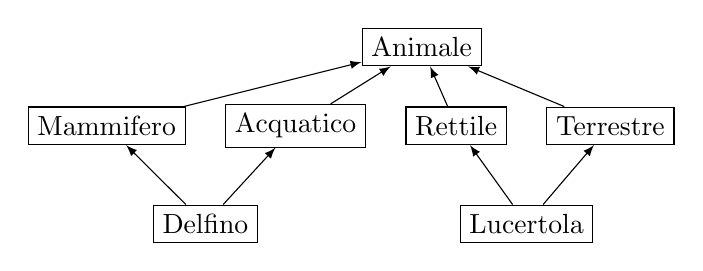
\begin{tikzpicture}
		\node [draw](Animale)at (0,0) {Animale};
		\node [draw](Mammifero)at (-4, -1) {Mammifero};
		\draw (Mammifero.east) ++ (0.5,0) node [draw, anchor = west](Acquatico) {Acquatico};
		\draw (Acquatico.east) ++ (0.5,0) node [draw, anchor = west](Rettile){Rettile};
		\draw (Rettile.east) ++ (0.5,0) node[draw, anchor = west](Terrestre){Terrestre};
		\path (Mammifero) -- (Acquatico) node (Delfino)[draw, midway, below, shift={(0,-1)} ]{Delfino};
		\path (Rettile) -- (Terrestre) node (Lucertola)[draw, midway, below, shift={(0,-1)} ]{Lucertola};
		\draw [-latex](Mammifero)--(Animale);
		\draw [-latex](Acquatico)--(Animale);
		\draw [-latex](Rettile)--(Animale);
		\draw [-latex](Terrestre)--(Animale);

		\draw [-latex](Delfino)--(Mammifero);
		\draw [-latex](Delfino)--(Acquatico);

		\draw [-latex](Lucertola)--(Rettile);
		\draw [-latex](Lucertola)--(Terrestre);
	\end{tikzpicture}
\end{center}
Un'ereditarietà di questo tipo \underline{non sarebbe} possibile in java, tuttavia lo è in linguaggi quali c++ o Python
%prova link \href{file:///Users/mattia/Desktop/prova.txt}{prova}
\subsection{Overriding}
Come abbiamo visto fin'ora, dire che una classe B estende una classe A, significa che B è una versione più dettagliata di A, una sua sottocategoria logica. A tutti gli effetti, B \textit{is a} A.

\begin{center}
	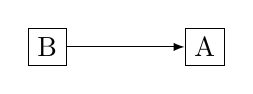
\begin{tikzpicture}
		\node (B)[draw]at (0,0) {B};
		\node (A)[draw]at (2,0) {A};
		\draw [-latex](B)--(A);
	\end{tikzpicture}
	\vskip3mm
	Si legge \textit{"B is a A"}
\end{center}
Per questa ragione in codice, supponendo di avere due classi:

\begin{lstlisting}[language = java, frame = none]
class A{
}

class B extends A{
}

\end{lstlisting}
\vskip3mm
possiamo scrivere delle cose di questo tipo
\vskip3mm
\begin{lstlisting}[language = java, frame = none]
  A a1 = new B();
  A a2 = new A();

  B b1 = new B();
\end{lstlisting}
\vskip3mm
occhio che la scrittura seguente è sbagliata (compiler error)
\vskip3mm
\begin{lstlisting}[language = java, frame = none]
  B b1 = new A(); //errore
\end{lstlisting}
\vskip3mm
\subsection{Overriding, overloading e polimorfismo}
Fino ad ora abbiamo visto come estendere classi e il significato dal punto di vista logico di questa operazione. Tuttavia l'ereditarietà ci permette di ricreare comportamenti molto più complessi tramite i meccanismi di overriding e overloading

\subsubsection{Overriding}
Nel momento in cui una classe $ B $ estende una classe $ A $, è possibile "sovrascrivere" un metodo di A in B, in modo tale da modificare il comportamento di quest'ultimo a seconda che venga utilizzato da un'istanza di tipo $ A $ o $ B $. Per utilizzare l'overriding devo ridefinire un metodo nella subclass, assicurandomi che questo abbia la  \footnote{Con signature o firma si intende il nome della funzione e i parametri presi in input}{\underline{stessa signature}} e stesso valore di ritorno. Supponiamo di avere:

\begin{lstlisting}[language = java, frame = none]

class A{
  void stampa(){
    System.out.println("Hello from A");
  }
}

class B extends A{
  void stampa(){
    System.out.println("Hello from B");
  }


\end{lstlisting}
\vskip3mm
Allora, all'interno del main posso fare qualcosa di questo tipo:
\vskip3mm
\begin{lstlisting}[language = java, frame = none]
      A a = new A();
      a.stampa();
      B b = new B();
      b.stampa();

      /*
      Hello from A
      Hello from B
      */
\end{lstlisting}

\subsubsection{Overloading}
L'overloading è un altro modo che abbiamo di far assumere comportamenti diversi al programma in base al contesto. Per utilizzare l'overloading devo creare due funzioni con lo stesso nome, ma parametri diversi. Anche il valore di ritorno può differire. Vediamo un esempio:
\vskip3mm

\begin{lstlisting}[language = java, frame = none]
public class Overloading {
  public static void main(String[] args) {
    stampa();
    stampa("Input");
    stampa(5);
    int v[] = {1,2,3,4,3,2,1};
    System.out.println(stampa(v));

  }

  public static void stampa() {
    System.out.println("0 argomenti");
  }

  public static void stampa(String text) {
    System.out.println("Stampo ciò che mi è stato dato in input:\n" + text + "\n");
  }

  public static void stampa(int x) {
    for (int i = 0; i < x; i++) {
      System.out.println(i + 1);
    }
  }

  public static int stampa(int v[]){
    System.out.println("");
    for(int x : v)
      System.out.print(x + " ");
    return v.length;
  }
}
\end{lstlisting}
\vskip3mm
Nota come
\begin{itemize}
	\item Le funzioni qui sono all'interno della stessa classe. Ciò che determina quale versione viene chiamata è il numero ed il tipo degli argomenti
	\item Il valore di ritorno può cambiare, tuttavia non può essere l'unica cosa diversa fra una funzione e l'altra (quale verisone chiamo?)
	\item Le funzioni \underline{non} devono necessariamente essere nella stessa classe
\end{itemize}
\subsubsection{Polimorfismo}
Overriding e overloading sono due metodi che abbiamo per applicare il concetto di \underline{polimorfismo}.
\begin{tcolorbox}
	In informatica, il termine polimorfismo (“avere molte forme”) viene usato in senso generico per riferirsi a espressioni  che possono rappresentare valori di diversi tipi  (dette espressioni polimorfiche).
\end{tcolorbox}

In particolare si può distinguere fra:
\begin{itemize}
	\item \underline{Polimorfismo sui dati}: informalmente, ciò che ci permette di fare \verb|A a = new B();| se B estende A
	\item \underline{Polimorfismo sui metodi}: ciò che possiamo ottenere tramite overloading e overriding.
\end{itemize}

%Per via della relazione logica fra queste classi, all'interno di un programma dovrebbe essere possibile sostituire un'istanza di una classe B con una di una classe A, nel momento in cui una estende l'altra. Questo è proprio ciò che enuncia il \underline{principio di sostituzione di Liskov}: 
%\bigbox{
%Data una classe B, sottoclasse di una classe A, dobbiamo essere in grado di passare un oggetto della classe B a qualsiasi metodo che si aspetti un oggetto della classe A, senza che il metodo restituisca un output inatteso.
%}
%Tutto questo è possibile in virtù del fatto che \textit{"B is a A"}
\subsection{Esercizi}

\begin{esercizio}{Gerarchia di animali}
	Scrivi del codice per rappresentare una gerarchia di animali. Le classi da rappresentare sono:
	\begin{itemize}
		\item {\ttfamily Animale}. Ha un {\ttfamily verso}, {\ttfamily peso},  {\ttfamily dimensione} e {\ttfamily sesso}. La dimensione è un enum che può assumere tre valori
		\item {\ttfamily Mammifero}
		\item {\ttfamily Rettile}
		\item {\ttfamily Delfino}
		\item {\ttfamily Lucertola}
	\end{itemize}
	Scrivere poi una funzione {\ttfamily toString}, che ritorni una stringa contenente le informazioni riguardo l'animale.
	\vskip3mm
	Implementare poi due classi: {\ttfamily cavallo} e {\ttfamily asino}. Creare una funzione {\ttfamily accoppia} che stampi a video il corretto incrocio:
	\begin{center}
		\begin{tabular}{ccc}
			\toprule
			      & cavallo  & cavalla \\
			\midrule
			asino & /        & mulo    \\
			asina & bardotto & /       \\
			\bottomrule
		\end{tabular}
	\end{center}

\end{esercizio}
\subsection{Tipo statico, dinamico e dynamic binding}
Fino ad ora, quando abbiamo parlato di "tipo" di una variabile ci siamo riferiti al tipo statico di questa. Tuttavia, supponendo che \verb|B extends A|, e dichiarando:
\begin{center}
	\verb|A x = new B();|
\end{center}
qual'è il tipo di \verb|x|?
\vskip3mm
Nel caso precedente, il tipo statico di \verb|x| è \verb|A|, mentre quello dinamico è \verb|B|. Potremmo quindi affermare che:
\begin{itemize}
	\item Il \underline{tipo statico}, o semplicemente "tipo", è il tipo indicato nella parte sinistra della dichiarazione della variabile
	\item Il \underline{tipo dinamico} è il tipo effettivo del valore contenuto nella variabile. Il tipo dinamico può cambiare infatti a \textit{runtime}
\end{itemize}

La possibilità di avere "un tipo dinamico", ci permette di creare comportamenti interessanti e talvolta difficili da capire, soprattutto tramite overriding e overloading
\subsubsection{Dynamic bining}
Partiamo vedendo i seguenti esempi di codice:

\begin{lstlisting}[language = java, frame = none]
public class es1 {

   public static void main(String[] args){
    A a = new B();
    a.stampa();
   }

}

class A {
  public void stampa(){
    System.out.println("A");
  }
}

class B extends A{
  public void stampa(){
    System.out.println("B");
  }
}
\end{lstlisting}
\vskip3mm
\vskip3mm
\begin{lstlisting}[language = java, frame = none]
  public class es2 {

  public static void main(String[] args) {
    A x = new B();
    stampa(x);
  }

  public static void stampa(A a) {
    System.out.println("A");
  }

  public static void stampa(B b) {
    System.out.println("A");
  }

}

class A {
}

class B extends A {
}
\end{lstlisting}
\vskip3mm
Quale sarà l'output in questi casi?
\vskip3mm
\begin{lstlisting}[language = java, frame = none]
public class es3 {

  public static void main(String[] args) {
    A x = new B();
    x.funcB();
  }

}

class A {
  public void funcA() {
    System.out.println("funcA");
  }
}

class B extends A {
  public void funcB() {
    System.out.println("funcB");
  }

}
\end{lstlisting}
\vskip3mm
In questo caso, invece, come mai ci viene dato un errore? Se invece apportassi una piccola modifica alla linea 5?
\begin{lstlisting}[language = java, frame = none]
public class es3 {

  public static void main(String[] args) {
    A x = new B();
    ((B)x).funcB();
  }

}

class A {
  public void funcA() {
    System.out.println("funcA");
  }
}

class B extends A {
  public void funcB() {
    System.out.println("funcB");
  }

}
\end{lstlisting}
Riassumendo i comportamenti mostrati in questi pezzi di codice possiamo dire che:
\begin{itemize}
	\item Il \underline{tipo statico determina}:
	      \begin{itemize}
		      \item Le funzioni che posso chiamare tramite un'istanza
		      \item L'overload che viene selezionato nel momento in cui una funzione prende in input una istanza
	      \end{itemize}
	\item Il \underline{tipo dinamico determina}:
	      \begin{itemize}
		      \item Quale override della funzione viene selezionato (fra tutti, viene chiamata l'override "più recente")
	      \end{itemize}
\end{itemize}
\subsubsection{Casting}
Nota che tramite casting io posso "forzare" il \underline{tipo statico} di una variabile. Se è una variabile di tipo \verb|A| ha un tipo dinamico \verb|B|, allora facendo il casting nel seguente modo posso accedere ai metodi e agli attributi dichiarati in \verb|B|. Posso ad esempio fare:
\begin{lstlisting}[language = java, frame = none]
public class es3 {

  public static void main(String[] args) {
    A x = new B();
    ((B)x).funcB();
  }

}

class A {
  public void funcA() {
    System.out.println("funcA");
  }
}

class B extends A {
  public void funcB() {
    System.out.println("funcB");
  }

}
\end{lstlisting}

\begin{tcolorbox}
	Attenzione: se si prova a castare una variabile ad un tipo dinamico che non coincide con quello corrente si ottiene un errore a runtime!
\end{tcolorbox}

\subsection{Esercizi}
\begin{enumerate}
	\item
	      \begin{lstlisting}[language = java, frame = none]
  public class Test {
    public static void main(String[] args) {
        A obj = new B();
        obj.m(new D());
    }
}
class A {
    void m(C c) { System.out.println("g"); }
}
class B extends A {
    void m(C c) { System.out.println("h"); }
    void m(D c) { System.out.println("i"); }
}
class C { }
class D extends C { }
\end{lstlisting}
	\item
	      \begin{lstlisting}[language = java, frame = none]
  public class Test {
    public static void main(String[] args) {
        A obj = new B();
        ((B)obj).m(new D());
    }
}
class A {
    void m(C c) { System.out.println("g"); }
}
class B extends A {
    void m(C c) { System.out.println("h"); }
    void m(D c) { System.out.println("i"); }
}
class C { }
class D extends C { }\end{lstlisting}
	\item 3
\end{enumerate}
\subsubsection{Link a esercizi carini}

\href{https://pg2.giuliopime.dev/home}{\textit{https://pg2.giuliopime.dev/home}}
\begin{itemize}
	\item Username: abbiamovinto
	\item Password: defacto
\end{itemize}
\href{https://training.olinfo.it}{\textit{https://training.olinfo.it}}
\subsection{Classi astratte}
Spesso, abbiamo bisogno di una classe che fornisca una "base", che vada poi espansa tramite altre classi che la estendono. Consideriamo ad esempio il class diagram seguente:

\begin{center}
	\begin{forest}
		for tree={edge={latex-}, draw}
		[Forma
			[Cerchio]
			[Quadrato]
			[Triangolo]
		]
	\end{forest}
\end{center}
In questo caso non ha senso avere un'istanza di tipo \verb|Forma|. Una forma, all'interno della nostra applicazione sarà sicuramente un \verb|Cerchio|, \verb|Quadrato| o \verb|Triangolo|. Per questo instanzieremo oggetti di questo tipo, non di tipo \verb|Forma|. In questa situazione ha senso che la classe \verb|Forma| sia astratta

\vskip3mm
La keyword \verb|abstract| può essere usata in due contesti:
\begin{itemize}
	\item Davanti alla definizione di una classe, per indicare che questa non può essere istanziata
	\item Davanti ad un metodo di una classe astratta, per indicare che questo non ha implementazione, ma verra overridato nelle classi che estenderanno la classe astratta
\end{itemize}

Un altro esempio di classe astratta può essere la classe \verb|Animale|, nel seguente contesto:
\begin{center}
	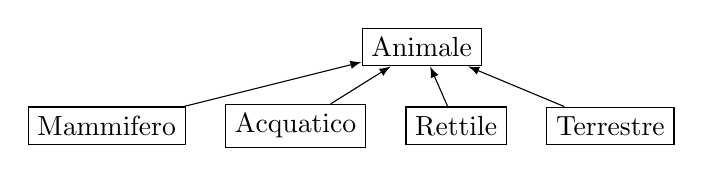
\begin{tikzpicture}
		\node [draw](Animale)at (0,0) {Animale};
		\node [draw](Mammifero)at (-4, -1) {Mammifero};
		\draw (Mammifero.east) ++ (0.5,0) node [draw, anchor = west](Acquatico) {Acquatico};
		\draw (Acquatico.east) ++ (0.5,0) node [draw, anchor = west](Rettile){Rettile};
		\draw (Rettile.east) ++ (0.5,0) node[draw, anchor = west](Terrestre){Terrestre};
		\draw [-latex](Mammifero)--(Animale);
		\draw [-latex](Acquatico)--(Animale);
		\draw [-latex](Rettile)--(Animale);
		\draw [-latex](Terrestre)--(Animale);
	\end{tikzpicture}
\end{center}
\subsubsection{Interfacce}
L'interfaccia è una sorta di \textit{"classe completamente astratta"}, ossia una classe i cui metodi \underline{non hanno implementazione}. In un certo senso, un'interfaccia ci permette di definire appunto dei metodi attraverso i quali possiamo \textit{interfacciarci} alla classe che la \underline{implementa}, la quale dovrà necessariamente fornire implementazione

\subsection{Esercizi}
\begin{esercizio}{Esercizio pokemon}
	Scrivere un programma che simuli il videogioco di pokemon

\end{esercizio}
Indizio: seguire il seguente \textit{class diagram}

\renewcommand{\umlfillcolor}{white}
\renewcommand{\umldrawcolor}{black}
{ \scriptsize

	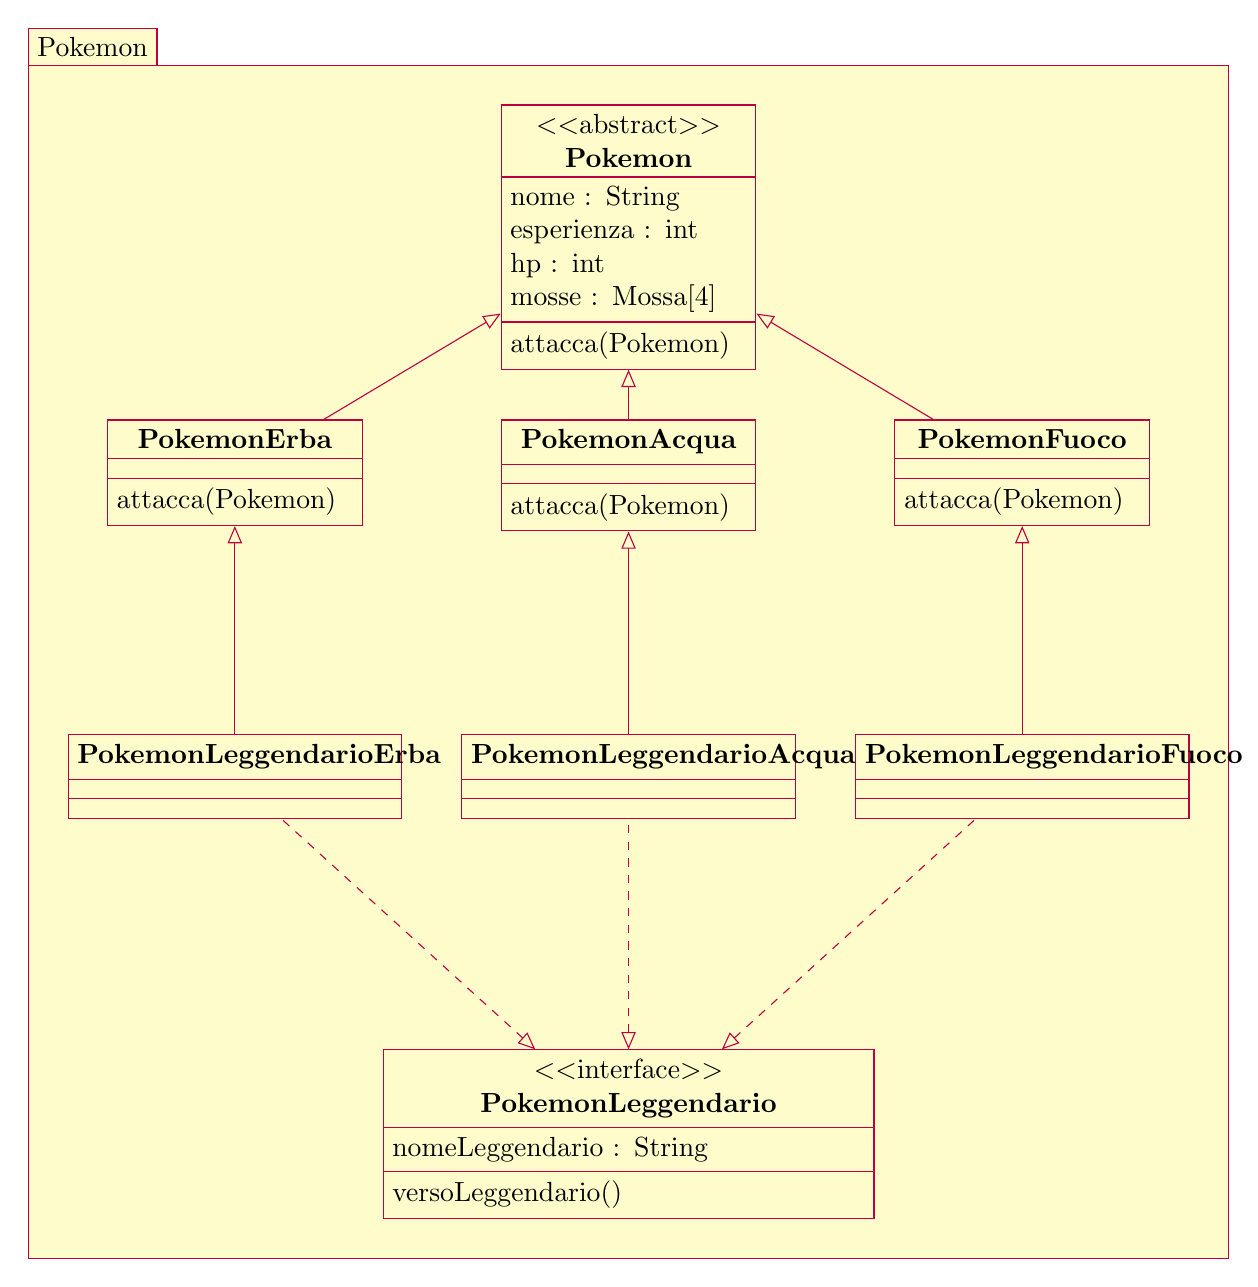
\begin{tikzpicture}
		\begin{package}{Pokemon}
			\begin{abstractclass}[text width = 3cm]{Pokemon}{0,0}
				\attribute{nome : String}
				\attribute{esperienza : int}
				\attribute{hp : int}
				\attribute{mosse : Mossa[4]}
				\operation{attacca(Pokemon)}
			\end{abstractclass}
			\begin{class}[text width = 3cm]{PokemonErba}{-5,-4}
				\inherit{Pokemon}
				\operation{attacca(Pokemon)}
			\end{class}
			\begin{class}[text width = 3cm]{PokemonAcqua}{0,-4}
				\inherit{Pokemon}
				\operation{attacca(Pokemon)}
			\end{class}
			\begin{class}[text width = 3cm]{PokemonFuoco}{5,-4}
				\inherit{Pokemon}
				\operation{attacca(Pokemon)}
			\end{class}

			\begin{interface}[text width = 6cm]{PokemonLeggendario}{0,-12}
				\attribute{nomeLeggendario : String}
				\operation{versoLeggendario()}
			\end{interface}
			\begin{class}[text width = 4cm]{PokemonLeggendarioErba}{-5,-8}
				\inherit{PokemonErba}
				\implement{PokemonLeggendario}
			\end{class}
			\begin{class}[text width = 4cm]{PokemonLeggendarioAcqua}{0,-8}
				\inherit{PokemonAcqua}
				\implement{PokemonLeggendario}
			\end{class}
			\begin{class}[text width = 4cm]{PokemonLeggendarioFuoco}{5,-8}
				\inherit{PokemonFuoco}
				\implement{PokemonLeggendario}
			\end{class}
		\end{package}


	\end{tikzpicture}

	\begin{center}
		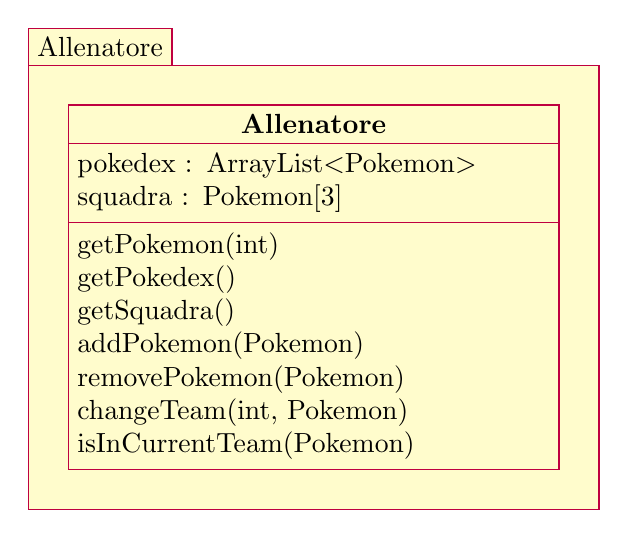
\begin{tikzpicture}
			\begin{package}{Allenatore}
				\begin{class}[text width = 6cm]{Allenatore}{0,0}
					\attribute{pokedex : ArrayList$ < $Pokemon$ > $}
					\attribute{squadra : Pokemon[3]}

					\operation{getPokemon(int)}
					\operation{getPokedex()}
					\operation{getSquadra()}
					\operation{addPokemon(Pokemon)}
					\operation{removePokemon(Pokemon)}
					\operation{changeTeam(int, Pokemon)}
					\operation{isInCurrentTeam(Pokemon)}
				\end{class}
			\end{package}
		\end{tikzpicture}
	\end{center}
}
\newpage



\section{Introduzione algoritmi}
Nella risoluzione di problemi di programmazione, spesso vengono utilizzate delle idee di base simili. Possiamo dire che gli algoritmi possono essere classificati in base al tipo di tecnica che utilizziamo per risolvere il problema.
\vskip3mm
Queste tecniche sono spesso indispensabili per questioni di efficienza (un algoritmo inefficiente potrebbe impiegare troppo tempo per essere eseguito, rendendolo inutilizzabile). Noi vedremo alcune delle più importanti

\subsection{Misurare l'efficienza}
I problemi di programmazione, tendenzialmente, non consistono in altro che implementare una funzione che, presi in input determinati dati, ne restituisce altri in output. Un fattore da importantissimo, da tenere in considerazione sempre, tuttavia, è \underline{la quantità di cicli di calcolo che il programma deve fare, in base all'input che ci viene dato}. Vediamo un esempio:

\begin{lstlisting}[language = java, frame = none]
  class esempio1 {
  public static void main(String[] args) {
    int v[] = { 1, 2, 3, 5, 2, 9, 11, -1 };
    System.out.println(massimo(v));
  }

  public static int massimo(int v[]) {
    int max = v[0];
    for (int i = 1; i < v.length; i++) {
      if (max < v[i])
        max = v[i];
    }

    return max;
  }
}

\end{lstlisting}

In questo caso, l'algoritmo(contenuto nella funzione \verb|massimo|) cerca il valore massimo nel vettore. Domande
\begin{itemize}
	\item Qual'è la dimensione dell'input?
	\item Se l'input è di dimensione $ n $, quanti cicli deve fare la funzione \verb|massimo|?
\end{itemize}
In questo caso, la dimensione dell'input è costituita dalla \underline{dimensione del vettore} \verb|v|, ossia 8.
\vskip3mm
Per come abbiamo scritto l'algoritmo, dato in input un vettore di dimensione 8, il ciclo verrà ripetuto 8 volte. Più in generale, \underline{dato un input un vettore di dimensione $ n $, l'algoritmo eseguirà $ n $ cicli} per restituire un risultato.
\begin{center}
	\tcbox{Formalmente, di dice che l'algoritmo che abbiamo scritto ha complessità $ O\left(n\right) $}
\end{center}
\subsection{Notazione $ O $}
Per indicare la complessità di un algoritmo, è molto usata la notazione $ O $ (\textit{big O}).
\begin{definizione}{Notazione big O}
	La notazione \textit{big O} serve per indicare la complessita di un algoritmo in funzione della dimensione del input che viene fornito al programma. In particolare, va indicata una funzione fra parentesi, che descrive il numero di cicli che il programma deve eseguire \underline{nel peggiore dei casi}, ad esempio:
	\[
		O\left(n\right) \quad O\left(n^2 \right) \quad O\left(n \log n\right) \quad O \left(\sqrt{n}\right)
	\]
\end{definizione}

Ad esempio, dire che un algoritmo ha complessità $ O\left(n^2 \right) $ significa che dato in input un dato di dimensione $ n $, impiegherà nel peggiore dei casi $ n^2  $ cicli per portare a termine l'esecuzione
\vskip3mm
Nella definizione data sopra, ci potrebberò essere 2 cose che creano dei dubbi:
\begin{itemize}
	\item Cosa significa che la notazione esprime il numero di cicli eseguiti \textit{"nel peggiore dei casi"}?
	\item Come va identificata la dimensione dell'input?
\end{itemize}

\subsubsection{Chiarificazione - "nel peggiore dei casi"}
Per rispondere alla prima domanda vediamo un frammento di codice:
\begin{lstlisting}[language = java, frame = none]
class esempio2 {
  public static void main(String[] args) {

    int v[] = { 1, 2, 3, 4, 5 };
    System.out.println(cointains(5, v));
    System.out.println(cointains(1, v));
    System.out.println(cointains(-2, v)); 
  }

  public static boolean cointains(int element, int v[]) {
    for (int i = 0; i < v.length; i++) {
      if (v[i] == element)
        return true;
    }
    return false;
  }
}
\end{lstlisting}

La funzione \verb|contains| ritorna true se \verb|element| è contenuto nell'array, altrimenti \verb|false|
\begin{itemize}
	\item Nella prima chiamata la funzione esegue 5 cicli
	\item Nella seconda chiamata la funzione esegue 1 solo ciclo
	\item Nell'ultima chiamata la funzion e esegue 5 cicli
\end{itemize}
Qual è la complessità dell'algoritmo?
\vskip3mm
Nonostante il numero di cicli cambi in base a come è formato l'input, l'algoritmo ha lo stesso complessità $ O\left(n\right) $, perché nel \underline{peggior caso}, dato un input di dimensione $ n $, esegue $ n $ cicli
\subsubsection{Dimensione dell'input}
La dimensione dell'input, non è necessariamente la lunghezza di un array, possiamo prendere come esempio il seguente algoritmo che somma tutti i numeri interi da 0 a $ n $:
\begin{lstlisting}[language = java, frame = none]
  
class esempio3 {
  public static void main(String[] args) {
    System.out.println(sumUpTo(10));
  }

  public static int sumUpTo(int n) {
    int sum = 0;

    for (int i = 1; i <= n; i++)
      sum += i;

    return sum;
  }
}
\end{lstlisting}
In questo caso, l'algoritmo ha complessità $ O\left(n\right) $, dove $ n $ però, non è la lunghezza di un vettore, ma il valore di $ n $, dato che è quello che influenza il numero di cicli eseguiti. Solitamente è evidente quale dimensione determina il numero di cicli eseguiti

\subsection{Complessità comuni}
La maggior parte di algoritmi ha una complessità fra le seguenti:
\vskip3mm
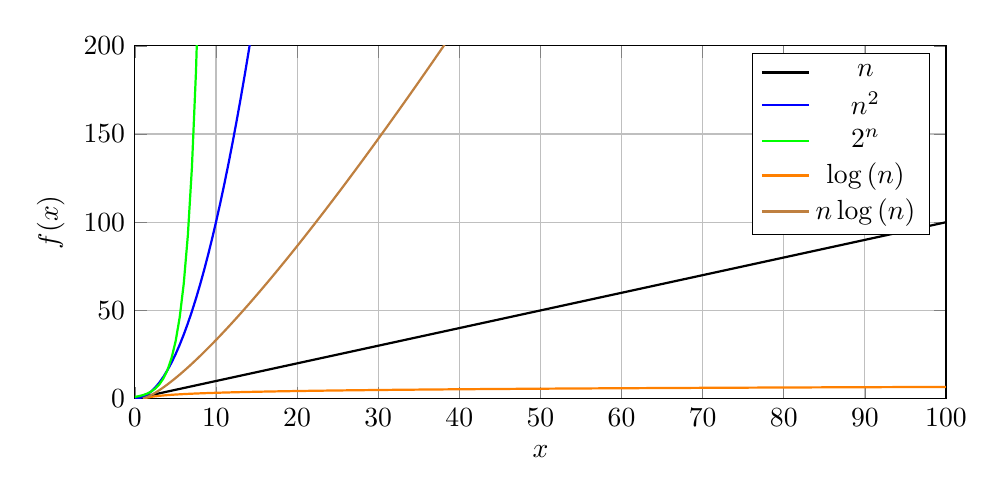
\begin{tikzpicture}
	\begin{axis}[
			xmin=0, xmax=100,
			ymin=0,ymax=200,
			restrict y to domain = 0:1000, domain=0:100, width=0.98\textwidth, height=0.5\textwidth, grid=major, samples=200,  ylabel=$f(x)$, xlabel=$x$, legend entries={$n$, $ n^2  $, $ 2^{n} $, $ \log \left(n\right) $, $ n \log \left(n\right) $}]
		\addplot[black, thick] {x};
		\addplot[blue, thick] {x^2};
		\addplot[green, thick] {2^x};
		\addplot[orange, thick] {ln(x)/ln(2)};
		\addplot[brown, thick] {x*(ln(x)/ln(2))};
	\end{axis}
\end{tikzpicture}
\vskip3mm

\addtocontents{exe}{\protect{\large \vskip3mm \textit{Algoritmi}\vskip3mm}}

\subsection{Esercizi di base}
\begin{esercizio}{Massimo vettore}
	Dato un vettore {\ttfamily v}, trovare l'elemento di valore massimo
\end{esercizio}

\begin{esercizio}{Compara stringhe 1}
	Date due array di caratteri {\ttfamily s1} e {\ttfamily s2}, ritornare {\ttfamily true} se sono uguali, {\ttfamily false} altrimenti
\end{esercizio}

\begin{esercizio}{Compara stringhe 2}
	Date due stringhe {\ttfamily s1} e {\ttfamily s2}, ritornare i seguenti valori:
	\begin{itemize}
		\item -1 se {\ttfamily s1} è alfabeticamente minore di {\ttfamily s2}
		\item 1 se {\ttfamily s1} è alfabeticamente maggiore di {\ttfamily s2}
		\item 0 se le stringhe sono uguali
	\end{itemize}

\end{esercizio}

\begin{esercizio}{Fattoriale}
	Dato in input un intero positivo {\ttfamily n}, se ne calcoli il fattoriale
\end{esercizio}

\begin{esercizio}{Massimo ricorsivo}
	Creare una funzione ricorsiva che trovi l'elemento massimo di un vettore
\end{esercizio}

\begin{esercizio}{Controllo contenuto vettore}
	Dati due vetttori {\ttfamily v1} e {\ttfamily v2} di dimensione uguale, ritornare {\ttfamily true} se contengono gli stessi elementi, {\ttfamily false} altrimenti (chiaramente, l'ordine degli elementi contenuti può cambiare)
	\vskip3mm
	Nota
	\begin{itemize}
		\item I vettori devono contenere gli stessi elementi \underline{nella stessa quantità}
		\item Si assuma che i valori contenuti nel vettore siano interi nel range $ \left[0,100\right) $
	\end{itemize}

	\renewcommand{\cellalign}{l}
	\begin{center}
		\begin{tabular}{lll}
			\toprule
			Input & Output & Discussione \\
			\midrule
			\makecell{v1: 1 1 1          \\v2: 1 1} & false & Stessi elementi ma in quantità diversa \\[12pt]
			\makecell{v1: 1 1 2 1 -5     \\v2: -5 1 2 1 1} & true & Stessi elementi nella steessa quantità \\
			\bottomrule
		\end{tabular}
	\end{center}

\end{esercizio}

\begin{esercizio}{Stampa matrice}
	Creare una funzione che presa in input una matrice di interi {\ttfamily m}, la stampi
\end{esercizio}

\begin{esercizio}{Inverti matrice}
	Creare una funzione che presa in input una matrice di interi {\ttfamily m}, ritorni un'altra matrice con righe e colonne invertite:
	\[
		\begin{bmatrix}
			1  & 2  & 3  & 4  & 5  \\
			6  & 7  & 8  & 9  & 10 \\
			11 & 12 & 13 & 14 & 15 \\
			16 & 17 & 18 & 19 & 20 \\
			21 & 22 & 23 & 24 & 25 \\
		\end{bmatrix}
		\rightarrow
		\begin{bmatrix}
			1 & 6  & 11 & 16 & 21 \\
			2 & 7  & 12 & 17 & 22 \\
			3 & 8  & 13 & 18 & 23 \\
			4 & 9  & 13 & 19 & 23 \\
			5 & 10 & 15 & 20 & 25 \\
		\end{bmatrix}
	\]

\end{esercizio}

\section{Programmazione dinamica}
Una delle tecniche più importanti, per risolvere problemi di programmazione, è detta \underline{programmazione dinamica}.
\vskip3mm
\begin{tcolorbox}
	La tecnica risolutiva della \underline{programmazione dinamica} consiste nella scomposizione di un problema in sottoproblemi più semplici i cui risultati vengono memorizzati e combinati per ottenere la soluzione del problem originario
\end{tcolorbox}

\vskip3mm
Dalla definizione questa tecnica sembra estremamente generica e vaga, vediamo degli esempi per rendere tutto più chiaro.
\subsubsection{Esempio programmazione dinamica 1}
Un esempio di problema risolvibile tramite programmazione dinamica è il calcolo del di un numero di fibonacci. La sequenza di fibonacci è così definita:
\[
	\text{Fib}\left(n\right) = \begin{cases}
		\text{Fib}\left(n-1\right) + \text{Fib}\left(n-2\right) & x>2   \\
		1                                                       & x = 2 \\
		0                                                       & x = 1
	\end{cases}
\]
\begin{lstlisting}[language = java, frame = none]
class esempio1 {
  public static void main(String[] args) {
    System.out.println(fibonacci(13));
  }

  public static int fibonacci(int n) {
    int fib[] = new int[n];
    fib[0] = 0;
    fib[1] = 1;
    for (int i = 2; i < n; i++) {
      fib[i] = fib[i - 1] + fib[i - 2];
    }

    return fib[n - 1];
  }
}
\end{lstlisting}

In questo è chiaro chiaro come possiamo salvare i risultati intermedi per poi riutilizzarrli: per calcolare $ \text{Fib}\left(n\right) $ utilizziamo $ \text{Fib}\left(n-1\right) $ e $ \text{Fib}\left(n-2\right) $ per questo salviamo tutti i risultati nel vettore \verb|fib|

\vskip3mm
Possiamo ora affrontare più formalmente i requisiti necessari per poter affrontare un problema tramite la tecnica della programmazione dinamica
\subsection{Quando affrontare un problema tramite programmazione dinamica}
A grandi linee, abbiamo bisogno che:
\begin{itemize}
	\item Il problema sia scomponibile in sottoproblemi più semplici da risolvere
	\item I sottoproblemi siano "sovrapposti" (\underline{overlapping subproblems}), ossia che la soluzione del sottoproblema $ n - 1$ serva per risolvere il sottoproblema $ n $
	\item Vi siano dei sottoproblemi che siano\textit{"casi base"}, la cui soluzione sia immediata. A partire da questi si possono costruire tutte le altre soluzioni
\end{itemize}
Collegando questi requisiti al prolema di fibonacci visto in precedenza, avremo che:
\begin{itemize}
	\item \underline{Sottoproblemi}: calcolo $\text{Fib}(n-1), \text{Fib}(n-2), \ldots , \text{Fib}\left(2\right), \text{Fib}\left(1\right)$
	\item \underline{Overlapping subproblems}: i problemi sono "overlapping" in quanto per calcolare $ \text{Fib}\left(n\right) $ ho bisogno di $ \text{Fib}\left(n-1\right) $ e $ \text{Fib}\left(n-2\right) $. Per risolvere un sottoproblema ho bisogno delle soluzioni di altri sottoproblemi
	\item \underline{Esistenza casi base}: nel caso in cui debba calcolare  $ \text{Fib}\left(1\right) $ e $ \text{Fib}\left(2\right) $ la soluzione è immediata
\end{itemize}

\addtocontents{exe}{\protect{\large \vskip3mm \textit{Problemi noti dp}\vskip3mm}}
\subsection{Problemi classici di programmazione dinamica}
\begin{esercizio}{Sottosequenza massima (Kadane's problem) \href{https://leetcode.com/problems/maximum-subarray}{(link)} }
	Dato in input un vettore {\ttfamily v}, contenente interi (anche negativi), si trovi la \footnote{Una sottosequenza è un insieme di elementi adiacenti all'interno del vettore}{sottosequenza} che abbia somma degli elementi massima. Si ritorni quest'ultima
	\vskip3mm
	\vskip3mm
	\underline{Input}
	\vskip3mm
	La dimensione $ n $ del vettore e sulla nuova riga gli elementi del vettore separati da uno spazio
	\vskip3mm
	\underline{Output}
	\vskip3mm
	La somma degli elementi della sottosequenza con somma massima
	\renewcommand{\cellalign}{l}
	\begin{center}
		\begin{tabularx}{\textwidth}{llX}
			\toprule
			Input & Output & Discussione \\
			\midrule
			\makecell{5                  \\ 1 2 3 4 5} & 15 & La sottosequenza è data dall'intero vettore \\
			\makecell{8                  \\ -2 -3 4 -1 -2 1 5 -3} & 7 & La sottosequenza è data dall'intervallo $ \left[2, 6\right] $ \\
			\makecell{4                  \\ -2 -3 -1 -11 } & 0 & Si assuma che la sottosequenza nulla abbia somma 0  \\
			\bottomrule
		\end{tabularx}
	\end{center}
	Complessità ottimale: $ O\left(v.size\right) $
\end{esercizio}
\vskip3mm

Un approccio naif sarebbe quello di generare tutte le sottosequenze possibili e confrontarne la somma, stampando quella massima. Questo approccio tuttavia sarebbe davvero inefficiente, tuttavia è molto semplice da implementare:
\begin{lstlisting}[language = java, frame = none]
    public static int subsequenceIneff(int v[]) {

    int max = 0;

    for (int i = 0; i < v.length; i++) {

      int currSum = 0;
      for (int j = i; j >= 0; j--) {
        currSum += v[j];
        if (currSum > max)
          max = currSum;
      }

    }

    return max;

  }
\end{lstlisting}
\[
	\text{ Complessità: } O\left(n^2 \right)
\]

Un approccio più efficiente può essere implementato tramite programmazione dinamica. L'idea è la seguente:
\begin{itemize}
	\item Salvo la sottosequenza con somma maggiore che finisce in posizione i-esima
	\item Calcolo la sottosequenza con somma maggiore che finisce in pos $ i+1 $ utilizzando la sottosequenza con somma maggiore che finisce in pos $ i $. Chiamiamo questo vettore \verb|dp|
\end{itemize}
Immaginiamo di salvarci i risultati intermedi in un vettore: questo vettore avrà dimensione $ n $ e conterrà in posizione $ i $ il sottovettore di somma massima che finisce in posizione $ i $. Notiamo innanzitutto che calcolare \verb|dp[0]| è scontato:
\begin{itemize}
	\item Se \verb|v[0] > 0| allora il sottovettore è costituito da un singolo elemento, ovvero \verb|v[0]|
	\item Se \verb|v[0] <= 0| allora il sottovettore è il sottovettore nullo, il quale ha sempre somma 0
\end{itemize}
Per calcolare invece \verb|dp[i]|, ragiono nel seguente modo:
\begin{itemize}
	\item Se \verb|dp[i-1] + v[i] > 0| allora \verb|dp[i] = dp[i-1] + v[i]| (mi conviene prendere la miglior sottosequenza che termina nella posizione prima e sommarci \verb|v[i]|, anche se questo è negativo)
	\item Se \verb|dp[i-1] + v[i] <=0| allora \verb|dp[i] = 0| (conviene "ripartire a formare il vettore", dato che concatenando la subsequence con somma maggiore che termina in $ i-1 $ aggiungerei solo una quantità negativa)
\end{itemize}
\begin{esercizio}{Cuttinig rod}
	Dato un cilindro di lunghezza {\ttfamily n} e un vettore {\ttfamily v} di dimensione {\ttfamily n}, che in {\ttfamily v[i]} contenga il prezzo di un cilindro lungo {\ttfamily i+1}, si stampi il prezzo massimo che posso ottenere tagliando il cilindro in quante parti voglio
	\vskip3mm
	\vskip3mm
	\underline{Input}
	\vskip3mm
	La dimensione $ n $(la lunghezza del cilindro) e sulla nuova riga gli $ n $ interi positivi che costituiscono gli elementi di v(ossia i prezzi di ogni taglio di cilindro)
	\vskip3mm
	\underline{Output}
	\vskip3mm
	Il prezzo massimo che posso ottenere suddividendo il cilindro
	\renewcommand{\cellalign}{l}
	\begin{center}
		\begin{tabularx}{\textwidth}{llX}
			\toprule
			Input & Output & Discussione \\
			\midrule
			\makecell{5                  \\ 1 2 3 4 5} & 5 & Posso tagliare il cilindro in molti modi per ottenere il valore 5:
			\vskip3mm
			\begin{center}
				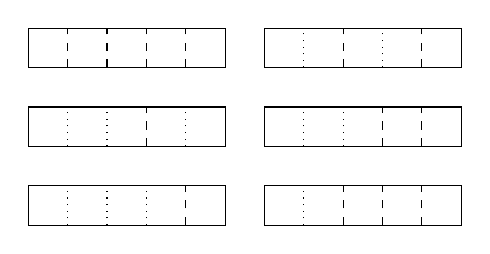
\begin{tikzpicture}[scale = 0.5]
					\draw (0,0)rectangle++(5,1);
					\foreach \x in {0,1,2,3,4,5}{
							\draw [dashed](0,0)++(\x,0)--(\x,1);
						}

					\draw (6,0)rectangle++(5,1);
					\foreach \x in {0,1,3,5}{
							\draw [dotted](6,0)++(\x,0)--++(0,1);
						}
					\draw [dashed](6,0)++(2,0)--++(0,1);
					\draw [dashed](6,0)++(4,0)--++(0,1);




					\draw (0,-2)rectangle++(5,1);
					\foreach \x in {0,1,2,4,5}{
							\draw [dotted](0,-2)++(\x,0)--++(0,1);
						}
					\draw [dashed](0,-2)++(3,0)--++(0,1);

					\draw (6,-2)rectangle++(5,1);
					\foreach \x in {0,1,2,5}{
							\draw [dotted](6,-2)++(\x,0)--++(0,1);
						}
					\draw [dashed](6,-2)++(3,0)--++(0,1);
					\draw [dashed](6,-2)++(4,0)--++(0,1);





					\draw (0,-4)rectangle++(5,1);
					\foreach \x in {0,1,2,3,5}{
							\draw [dotted](0,-4)++(\x,0)--++(0,1);
						}

					\draw [dashed](0,-4)++(4,0)--++(0,1);
					\draw (6,-4)rectangle++(5,1);
					\foreach \x in {0,1}{
							\draw [dotted](6,-4)++(\x,0)--++(0,1);
						}
					\draw [dashed](6,-4)++(4,0)--++(0,1);
					\draw [dashed](6,-4)++(3,0)--++(0,1);
					\draw [dashed](6,-4)++(2,0)--++(0,1);

				\end{tikzpicture}
			\end{center}
			\\
			\midrule
			\makecell{7                  \\ 1 4 10 8 5 10 13} & 21 & In questo caso ciò che conviene fare è spezzare il cilindro in 2 pezzi di lunghezza 3 e 1 di lunghezza 1:

			\begin{center}
				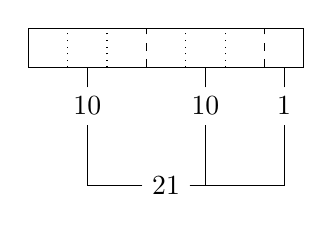
\begin{tikzpicture}[scale = 0.5]
					\draw (0,0)rectangle++(7,1);
					\foreach \x in {0,1,2,4,5,7}{
							\draw [dotted](0,0)++(\x,0)--(\x,1);
						}
					\draw [dashed](3,0)--++(0,1);
					\draw [dashed](6,0)--++(0,1);

					\node (a)[anchor = north] at(1.5, -0.5)  {10};
					\node (b)[anchor = north] at(4.5, -0.5)  {10};
					\node (c)[anchor = north] at(6.5, -0.5)  {1};
					\draw (a.north)--++(0,0.5);
					\draw (b.north)--++(0,0.5);
					\draw (c.north)--++(0,0.5);

					\node (d)at(3.5, -3)  {21};
					\draw (d)-|(a);
					\draw (d)-|(b);
					\draw (d)-|(c);

				\end{tikzpicture}
			\end{center}
			\\
			\bottomrule
		\end{tabularx}
	\end{center}
	Complessità ottimale: $ O\left(n \cdot v.size\left(\right)\right) $
\end{esercizio}\label{cuttingrod}

L'idea di base per risolvere il problema è la seguente:
\begin{itemize}
	\item Creo un vettore \verb|dp| all'interno del quale salvo \underline{nella $ i $-\textit{esima} cella il valore massimo che posso ottenere suddividendo un cilindro di lunghezza $ i+1 $}
	\item Costruisco il vettore \verb|dp| partendo dal caso base: \verb|dp[0] = prezzi [0]|, in quanto ho un solo modo di suddividere un cilindro lungo 1
	\item Contanto sul fatto che il vettore \verb|dp| contenga il \underline{il prezzo maggiore che posso ottenere suddividendo il cilindro in un dato modo}, calcolo \verb|dp[i+1]| sfruttando i dati contenuti nelle celle precedenti del vettore \verb|dp|.In particolare, supponendo di dover calcolare la posizione $ i $ del vettore \verb|dp|, devo:
	      \begin{itemize}
		      \item Calcolare il prezzo che otterrei mettendo in posizione $ i $ un pezzo di ogni lunghezza, da 1 a $ i $
		      \item Confrontare i prezzi ottenuti
		      \item \verb|dp[i]| è il valore massimo fra questi prezzi
	      \end{itemize}
\end{itemize}
Vediamo un esempio grafico. Supponiamo di avere in input il vettore \verb|prezzi|, con valori:
\begin{center}
	1 4 10 8 5 10 13
\end{center}
Ripercorriamo gli step appena descritti.

\begin{itemize}
	\item Creo un vettore \verb|dp| all'interno del quale salvo \underline{nella $ i $-\textit{esima} cella il valore massimo che posso ottenere suddividendo un cilindro di lunghezza $ i+1 $}
	\item Costruisco il vettore \verb|dp| partendo dal caso base: \verb|dp[0] = prezzi [0]|, in quanto ho un solo modo di suddividere un cilindro lungo 1. Quindi nel nostro caso:

	      \begin{center}
		      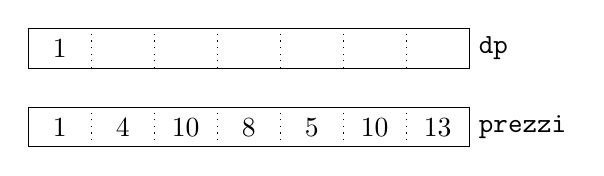
\begin{tikzpicture}[yscale = 0.5, xscale = 0.8]
			      \draw (0,-2)rectangle++(7,1);
			      \foreach \x in {0,1,2,3,4,5,6,7}{
					      \draw [dotted](0,-2)++(\x,0)--++(0,1);
				      }
			      \node  at (0.5,-1.5)  {1};
			      \node  at (1.5,-1.5)  {4};
			      \node  at (2.5,-1.5)  {10};
			      \node  at (3.5,-1.5)  {8};
			      \node  at (4.5,-1.5)  {5};
			      \node  at (5.5,-1.5)  {10};
			      \node  at (6.5,-1.5)  {13};

			      \node  [anchor = west] at (7,-1.5)  {\ttfamily prezzi};


			      \draw (0,0)rectangle++(7,1);
			      \foreach \x in {0,1,2,3,4,5,6,7}{
					      \draw [dotted](0,0)++(\x,0)--(\x,1);
				      }
			      \node  at (0.5,0.5)  {1};
			      \node  [anchor = west] at (7,0.5)  {\ttfamily dp};

		      \end{tikzpicture}
	      \end{center}

	      Chiaramente, un cilindro id lunghezza 1 non può essere suddiviso, quindi l'unico prezzo possibile è il prezzo del cilindro lungo 1, ossia 1 nel nostro caso


	\item Contanto sul fatto che il vettore \verb|dp| contenga il \underline{il prezzo maggiore che posso ottenere suddividendo il cilindro in un dato modo}, calcolo \verb|dp[i+1]| sfruttando i dati contenuti nelle celle precedenti del vettore \verb|dp|.In particolare, supponendo di dover calcolare la posizione $ i $ del vettore \verb|dp|, devo:
	      \begin{itemize}
		      \item Calcolare il prezzo che otterrei mettendo in posizione $ i $ un pezzo di ogni lunghezza, da 1 a $ i $
		      \item Confrontare i prezzi ottenuti
		      \item \verb|dp[i]| è il valore massimo fra questi prezzi
	      \end{itemize}
	      Iniziamo quindi calcolando \verb|v[1]|. So di avere già calcolato il prezzo migliore per suddividere un cilindro di lunghezza $ 1 $. Quindi per arrivare ad avere un cilindro di lunghezza 2 ho due alternative:

	      \begin{center}
		      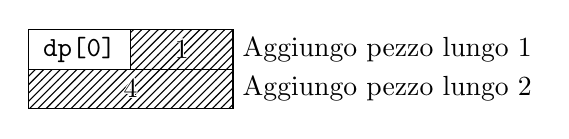
\begin{tikzpicture}[yscale = 0.5, xscale = 1.3]


			      \draw (0,2)rectangle++(2,2);
			      \draw (0,3)--(2,3);

			      \node ()[anchor = west]at (2,3.5) {Aggiungo pezzo lungo 1};
			      \node ()[anchor = west]at (2,2.5) {Aggiungo pezzo lungo 2};

			      \draw [pattern = north east lines](1,3)rectangle(2,4);
			      \draw [pattern = north east lines](0,2)rectangle(2,3);

			      \node () at (0.5,3.5)  {\ttfamily dp[0]};
			      \node () at (1.5,3.5)  {\contour{white}{1}};

			      \node () at (1, 2.5)  {\contour{white}{4}};

		      \end{tikzpicture}
	      \end{center}
	      Ora devo decidere se mi convenga prendere un solo cilindro da 2 oppure suddividerlo in due pezzi da 1. Mi basta però vedere quale delle opzioni ha prezzo maggiore. In questo caso conviene prendere un pezzo da 2 con costo 4. Dp diventa:

	      \begin{center}
		      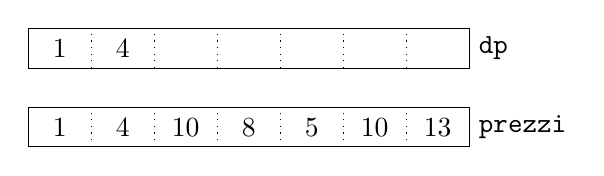
\begin{tikzpicture}[yscale = 0.5, xscale = 0.8]
			      \draw (0,0)rectangle++(7,1);
			      \foreach \x in {0,1,2,3,4,5,6,7}{
					      \draw [dotted](0,0)++(\x,0)--(\x,1);
				      }


			      \node  at (0.5,0.5)  {1};
			      \node  at (1.5,0.5)  {4};
			      \node  [anchor = west] at (7,0.5)  {\ttfamily dp};

			      \draw (0,-2)rectangle++(7,1);
			      \foreach \x in {0,1,2,3,4,5,6,7}{
					      \draw [dotted](0,-2)++(\x,0)--++(0,1);
				      }
			      \node  at (0.5,-1.5)  {1};
			      \node  at (1.5,-1.5)  {4};
			      \node  at (2.5,-1.5)  {10};
			      \node  at (3.5,-1.5)  {8};
			      \node  at (4.5,-1.5)  {5};
			      \node  at (5.5,-1.5)  {10};
			      \node  at (6.5,-1.5)  {13};

			      \node  [anchor = west] at (7,-1.5)  {\ttfamily prezzi};

		      \end{tikzpicture}
	      \end{center}

	      Ripetiamo il passaggio per $ i=3 $
\end{itemize}

\newcommand{\dpvector}{
	\def\rows{1}
	\def\columns{7}
	\def\shiftx{0}
	\def\shifty{-2}


	\foreach \x in {0,1,...,\columns}{
			\draw [dotted](0 + \shiftx,0 + \shifty)++(\x,0)--++(0,\rows);
		}

	\draw (\shiftx, \shifty)rectangle++(\columns, \rows);

	\node ()[anchor = west]at(7,-1.5) {\ttfamily dp};
}

\begin{minipage}[t]{0.48\textwidth}
	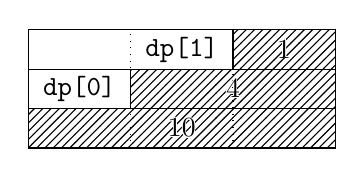
\begin{tikzpicture}[yscale = 0.5, xscale = 1.3]


		\def\rows{3}
		\def\columns{3}
		\newcommand{\shiftx}{0}
		\newcommand{\shifty}{0}


		\foreach \x in {0,1,...,\columns}{
				\draw [dotted](0 + \shiftx,0 + \shifty)++(\x,0)--++(0,\rows);
			}

		\foreach \x in {0,1,...,\rows}{
				\draw (0 + \shiftx,0 + \shifty)++(0,\x)--++(\columns,0);
			}

		\draw (\shiftx, \shifty)rectangle++(\columns, \rows);


		\foreach \x in {\rows,...,1}{
				\draw [pattern = north east lines](\shiftx + \columns - \x,\shifty + \rows - \x)rectangle++(\x, );
			}


		\node ()at (2.5, 2.5)  {\contour{white}{1}};
		\node ()at (2, 1.5)  {\contour{white}{4}};
		\node ()at (1.5, 0.5)  {\contour{white}{10}};

		\node ()at(1.5,2.5)  {\ttfamily dp[1]};
		\node ()at(0.5,1.5)  {\ttfamily dp[0]};




	\end{tikzpicture}
	\vskip3mm
	\begin{tikzpicture}[yscale = 0.5, xscale = 0.8]

		\dpvector

		\node ()at(0.5,-1.5) {1};
		\node ()at(1.5,-1.5) {4};
		\node ()at(2.5,-1.5) {\textcolor{gray}{10}};
	\end{tikzpicture}
\end{minipage}
%
\begin{minipage}[t]{0.48\textwidth}

	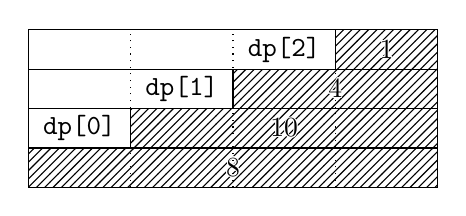
\begin{tikzpicture}[yscale = 0.5, xscale = 1.3]
		\def\rows{4}
		\def\columns{4}
		\newcommand{\shiftx}{0}
		\newcommand{\shifty}{0}


		\foreach \x in {0,1,...,\columns}{
				\draw [dotted](0 + \shiftx,0 + \shifty)++(\x,0)--++(0,\rows);
			}

		\foreach \x in {0,1,...,\rows}{
				\draw (0 + \shiftx,0 + \shifty)++(0,\x)--++(\columns,0);
			}

		\draw (\shiftx, \shifty)rectangle++(\columns, \rows);


		\foreach \x in {\rows,...,1}{
				\draw [pattern = north east lines](\shiftx + \columns - \x,\shifty + \rows - \x)rectangle++(\x, );
			}

		\node ()at (3.5, 3.5)  {\contour{white}{1}};
		\node ()at (3, 2.5)  {\contour{white}{4}};
		\node ()at (2.5, 1.5)  {\contour{white}{10}};
		\node ()at (2, 0.5)  {\contour{white}{8}};

		\node ()at(2.5,3.5)  {\ttfamily dp[2]};
		\node ()at(1.5,2.5)  {\ttfamily dp[1]};
		\node ()at(0.5,1.5)  {\ttfamily dp[0]};
	\end{tikzpicture}
	\vskip3mm
	\begin{tikzpicture}[yscale = 0.5, xscale = 0.8]

		\dpvector

		\node ()at(0.5,-1.5) {1};
		\node ()at(1.5,-1.5) {4};
		\node ()at(2.5,-1.5) {10};
		\node ()at(3.5,-1.5) {\textcolor{gray}{11}};
	\end{tikzpicture}
\end{minipage}


\vskip20mm


%
\begin{minipage}[t]{0.48\textwidth}
	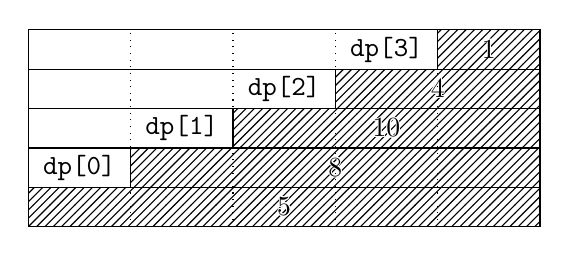
\begin{tikzpicture}[yscale = 0.5, xscale = 1.3]
		\def\rows{5}
		\def\columns{5}
		\newcommand{\shiftx}{0}
		\newcommand{\shifty}{0}


		\foreach \x in {0,1,...,\columns}{
				\draw [dotted](0 + \shiftx,0 + \shifty)++(\x,0)--++(0,\rows);
			}

		\foreach \x in {0,1,...,\rows}{
				\draw (0 + \shiftx,0 + \shifty)++(0,\x)--++(\columns,0);
			}

		\draw (\shiftx, \shifty)rectangle++(\columns, \rows);


		\foreach \x in {\rows,...,1}{
				\draw [pattern = north east lines](\shiftx + \columns - \x,\shifty + \rows - \x)rectangle++(\x, );
			}

		\node ()at (4.5, 4.5)  {\contour{white}{1}};
		\node ()at (4, 3.5)  {\contour{white}{4}};
		\node ()at (3.5, 2.5)  {\contour{white}{10}};
		\node ()at (3, 1.5)  {\contour{white}{8}};
		\node ()at (2.5, 0.5)  {\contour{white}{5}};

		\node ()at(3.5,4.5)  {\ttfamily dp[3]};
		\node ()at(2.5,3.5)  {\ttfamily dp[2]};
		\node ()at(1.5,2.5)  {\ttfamily dp[1]};
		\node ()at(0.5,1.5)  {\ttfamily dp[0]};
	\end{tikzpicture}
	\vskip3mm
	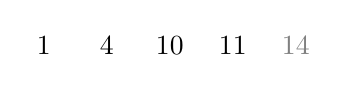
\begin{tikzpicture}[yscale = 0.5, xscale = 0.8]

		\dpvector

		\node ()at(0.5,-1.5) {1};
		\node ()at(1.5,-1.5) {4};
		\node ()at(2.5,-1.5) {10};
		\node ()at(3.5,-1.5) {11};
		\node ()at(4.5,-1.5) {\textcolor{gray}{14}};
	\end{tikzpicture}
\end{minipage}
%
\begin{minipage}[t]{0.48\textwidth}
	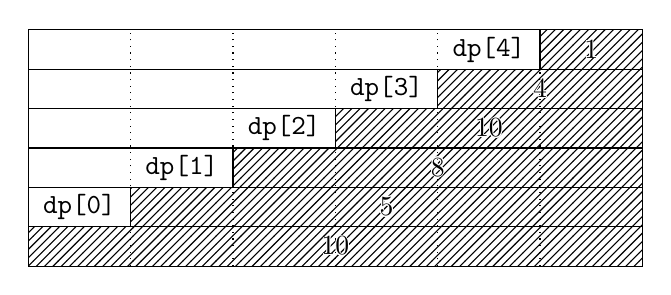
\begin{tikzpicture}[yscale = 0.5, xscale = 1.3]
		\def\rows{6}
		\def\columns{6}
		\newcommand{\shiftx}{0}
		\newcommand{\shifty}{0}


		\foreach \x in {0,1,...,\columns}{
				\draw [dotted](0 + \shiftx,0 + \shifty)++(\x,0)--++(0,\rows);
			}

		\foreach \x in {0,1,...,\rows}{
				\draw (0 + \shiftx,0 + \shifty)++(0,\x)--++(\columns,0);
			}

		\draw (\shiftx, \shifty)rectangle++(\columns, \rows);


		\foreach \x in {\rows,...,1}{
				\draw [pattern = north east lines](\shiftx + \columns - \x,\shifty + \rows - \x)rectangle++(\x, );
			}

		\node ()at (5.5, 5.5)  {\contour{white}{1}};
		\node ()at (5, 4.5)  {\contour{white}{4}};
		\node ()at (4.5, 3.5)  {\contour{white}{10}};
		\node ()at (4, 2.5)  {\contour{white}{8}};
		\node ()at (3.5, 1.5)  {\contour{white}{5}};
		\node ()at (3, 0.5)  {\contour{white}{10}};

		\node ()at(4.5,5.5)  {\ttfamily dp[4]};
		\node ()at(3.5,4.5)  {\ttfamily dp[3]};
		\node ()at(2.5,3.5)  {\ttfamily dp[2]};
		\node ()at(1.5,2.5)  {\ttfamily dp[1]};
		\node ()at(0.5,1.5)  {\ttfamily dp[0]};
	\end{tikzpicture}
	\vskip3mm
	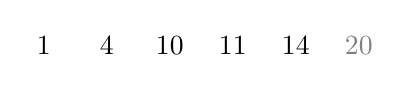
\begin{tikzpicture}[yscale = 0.5, xscale = 0.8]

		\dpvector

		\node ()at(0.5,-1.5) {1};
		\node ()at(1.5,-1.5) {4};
		\node ()at(2.5,-1.5) {10};
		\node ()at(3.5,-1.5) {11};
		\node ()at(4.5,-1.5) {14};
		\node ()at(5.5,-1.5) {\textcolor{gray}{20}};
	\end{tikzpicture}

\end{minipage}

\vskip15mm

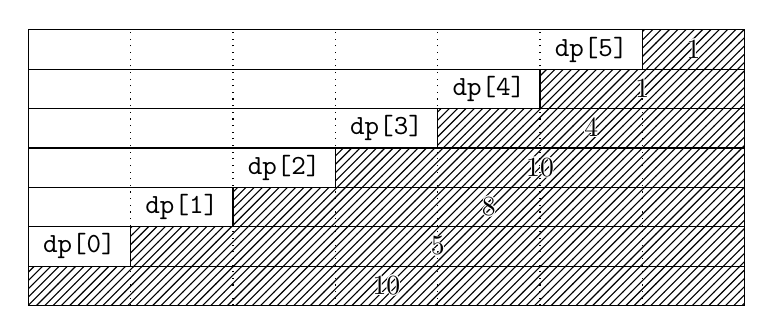
\begin{tikzpicture}[yscale = 0.5, xscale = 1.3]
	\def\rows{7}
	\def\columns{7}
	\newcommand{\shiftx}{0}
	\newcommand{\shifty}{0}


	\foreach \x in {0,1,...,\columns}{
			\draw [dotted](0 + \shiftx,0 + \shifty)++(\x,0)--++(0,\rows);
		}

	\foreach \x in {0,1,...,\rows}{
			\draw (0 + \shiftx,0 + \shifty)++(0,\x)--++(\columns,0);
		}

	\draw (\shiftx, \shifty)rectangle++(\columns, \rows);


	\foreach \x in {\rows,...,1}{
			\draw [pattern = north east lines](\shiftx + \columns - \x,\shifty + \rows - \x)rectangle++(\x, );
		}

	\node ()at (6.5, 6.5)  {\contour{white}{1}};
	\node ()at (6, 5.5)  {\contour{white}{1}};
	\node ()at (5.5, 4.5)  {\contour{white}{4}};
	\node ()at (5, 3.5)  {\contour{white}{10}};
	\node ()at (4.5, 2.5)  {\contour{white}{8}};
	\node ()at (4, 1.5)  {\contour{white}{5}};
	\node ()at (3.5, 0.5)  {\contour{white}{10}};

	\node ()at(5.5,6.5)  {\ttfamily dp[5]};
	\node ()at(4.5,5.5)  {\ttfamily dp[4]};
	\node ()at(3.5,4.5)  {\ttfamily dp[3]};
	\node ()at(2.5,3.5)  {\ttfamily dp[2]};
	\node ()at(1.5,2.5)  {\ttfamily dp[1]};
	\node ()at(0.5,1.5)  {\ttfamily dp[0]};
\end{tikzpicture}
\vskip3mm
\begin{tikzpicture}[yscale = 0.5, xscale = 1.3]

	\dpvector

	\node ()at(0.5,-1.5) {1};
	\node ()at(1.5,-1.5) {4};
	\node ()at(2.5,-1.5) {10};
	\node ()at(3.5,-1.5) {11};
	\node ()at(4.5,-1.5) {14};
	\node ()at(5.5,-1.5) {20};
	\node ()at(6.5,-1.5) {\textcolor{gray}{21}};
\end{tikzpicture}


\begin{esercizio}{Somma e media \href{https://training.olinfo.it/\#/task/array/statement}{(link)}}
	Dati in input un numero $ N $, e successivamente $ N $ interi, calcolare la media aritmetica e la somma di questi ultimi
	\vskip3mm
	\underline{Input:}
	\vskip3mm Sulla prima riga l'intero $ N $, sulla seconda riga $ N $ interi separati da uno spazio
	\vskip3mm
	\underline{Output:}
	\vskip3mm Due interi: rispettivamente la somma degli $ N $ numeri e la loro media aritmetica
	\renewcommand{\cellalign}{l}
	\vskip3mm
	\begin{tabularx}{\textwidth}{llX}
		\toprule
		Input & Output & Discussione \\
		\midrule
		\makecell{1                  \\ 12} & 5 & Somma e media coincidono e hanno valore 12\\[12pt]
		\makecell{7                  \\ 1 2 34 -56 33 23 89} & 126 18 & Somma e media coincidono e hanno valore 12\\
		\bottomrule
	\end{tabularx}
	\vskip3mm
	Complessità ottimale: $ O\left(N\right) $
\end{esercizio}

\begin{esercizio}{Majority element \href{https://leetcode.com/problems/majority-element/submissions/}{(link)}}
	Dato un array \textit{nums} di dimentione $ n $, ritornare il \textit{majority element}. Il \textit{majority element} è l'elemento che appare \underline{di più} di $ \frac{n}{2} $ volte. Si può assumere che l'elemento esista sempre nell'array
	\vskip3mm
	\underline{Input:}
	\vskip3mm Sulla prima riga l'intero $ n $, sulla seconda riga $ n $, ossia gli elementi di \textit{nums}
	\vskip3mm
	\underline{Output:}
	\vskip3mm Un intero, il majority element
	\vskip3mm
	\renewcommand{\cellalign}{l}
	\begin{tabularx}{\textwidth}{llX}
		\toprule
		Input & Output & Discussione \\
		\midrule
		\makecell{3                  \\ 3 2 3} & 3 & 3 appare più di 3/2 = 1 volta \\[12pt]
		\makecell{7                  \\ 2 2 1 1 1 2 2} & 2 & 2 appare più di 7/2 = 3 volte\\
		\bottomrule
	\end{tabularx}
	\vskip3mm
	Complessità ottimale: $ O\left(n\right) $
\end{esercizio}

\begin{esercizio}{Longest Common Subsequence \href{https://leetcode.com/problems/longest-common-subsequence/}{(link)}}
	Date in input due stringhe \textit{S1} ed \textit{S2}, si ritorni la lunghezza della \textit{longhest common subsequence}, ossia della \footnote{Con \underline{sottoseuquenza} si intende la una stringa che si può ottenere da un'altra eliminando determinati caratteri: \textit{bedbreakfast} è una sottosequenza di \textit{bedandbreakfast}. A differenza di ciò che accade in un \underline{sottovettore}, i caratteri \underline{non} devono essere necessariamente contigui: \textit{bedbreakfast} è sottosequenza ma non sottovettore; \textit{breakfast} è sottosequenza e sottovettore}{sottosequenza} più lunga comunque ad esntrambe le stringhe.
	\vskip3mm
	\underline{Input:}
	\vskip3mm Due stringhe, una per riga, composte da caratteri maiuscoli compresi fra $ A $ e $ Z $
	\vskip3mm
	\underline{Output:}
	\vskip3mm Un intero, la lunghezza della più lunga sottosequenza comune ad entrambe le stringhe
	\vskip3mm
	\renewcommand{\cellalign}{l}
	\begin{tabularx}{\textwidth}{llX}
		\toprule
		Input & Output & Discussione \\
		\midrule
		\makecell{AGGTAB             \\GXTXAYB} & 4 & La sottosequenza comune con lunghezza maggiore è \textit{"GTAB"}, ed ha lunghezza pari a 4  \\[12pt]
		\makecell{AABBCCD            \\  AABBD} & 5 & La sottosequenza comune con lunghezza maggiore è \textit{"AABBD", ed ha lunghezza pari a 5}\\
		\bottomrule
	\end{tabularx}
	\vskip3mm
	Complessità ottimale: $ O\left(s_1.lenght \cdot s_2.lenght\right) $
\end{esercizio}
Per risolvere questo problema dobbiamo utilizzare una matrice di supporto, che salverà i valori intermedi e ci permetterà di utilizzare la programmazione dinamica. Prendiamo come esempio il le stringhe \textit{"AGGTAB"} e \textit{"GXTXAYB"}. La matrice di supporto deve avere la seguente forma:
\begin{center}
	\begin{tabular}{cccccccccl}
		                          &                        & G                      & X                      & T                      & X                      & A                      & Y                      & B                      & s1, j \\ \cline{2-9}
		\multicolumn{1}{c|}{}     & \multicolumn{1}{c|}{0} & \multicolumn{1}{c|}{0} & \multicolumn{1}{c|}{0} & \multicolumn{1}{c|}{0} & \multicolumn{1}{c|}{0} & \multicolumn{1}{c|}{0} & \multicolumn{1}{c|}{0} & \multicolumn{1}{c|}{0} &       \\ \cline{2-9}
		\multicolumn{1}{c|}{A}    & \multicolumn{1}{c|}{0} & \multicolumn{1}{c|}{}  & \multicolumn{1}{c|}{}  & \multicolumn{1}{c|}{}  & \multicolumn{1}{c|}{}  & \multicolumn{1}{c|}{}  & \multicolumn{1}{c|}{}  & \multicolumn{1}{c|}{}  &       \\ \cline{2-9}
		\multicolumn{1}{c|}{G}    & \multicolumn{1}{c|}{0} & \multicolumn{1}{c|}{}  & \multicolumn{1}{c|}{}  & \multicolumn{1}{c|}{}  & \multicolumn{1}{c|}{}  & \multicolumn{1}{c|}{}  & \multicolumn{1}{c|}{}  & \multicolumn{1}{c|}{}  &       \\ \cline{2-9}
		\multicolumn{1}{c|}{G}    & \multicolumn{1}{c|}{0} & \multicolumn{1}{c|}{}  & \multicolumn{1}{c|}{}  & \multicolumn{1}{c|}{}  & \multicolumn{1}{c|}{}  & \multicolumn{1}{c|}{}  & \multicolumn{1}{c|}{}  & \multicolumn{1}{c|}{}  &       \\ \cline{2-9}
		\multicolumn{1}{c|}{T}    & \multicolumn{1}{c|}{0} & \multicolumn{1}{c|}{}  & \multicolumn{1}{c|}{}  & \multicolumn{1}{c|}{}  & \multicolumn{1}{c|}{}  & \multicolumn{1}{c|}{}  & \multicolumn{1}{c|}{}  & \multicolumn{1}{c|}{}  &       \\ \cline{2-9}
		\multicolumn{1}{c|}{A}    & \multicolumn{1}{c|}{0} & \multicolumn{1}{c|}{}  & \multicolumn{1}{c|}{}  & \multicolumn{1}{c|}{}  & \multicolumn{1}{c|}{}  & \multicolumn{1}{c|}{}  & \multicolumn{1}{c|}{}  & \multicolumn{1}{c|}{}  &       \\ \cline{2-9}
		\multicolumn{1}{c|}{B}    & \multicolumn{1}{c|}{0} & \multicolumn{1}{c|}{}  & \multicolumn{1}{c|}{}  & \multicolumn{1}{c|}{}  & \multicolumn{1}{c|}{}  & \multicolumn{1}{c|}{}  & \multicolumn{1}{c|}{}  & \multicolumn{1}{c|}{}  &       \\ \cline{2-9}
		\multicolumn{1}{l}{s2, i} & \multicolumn{1}{l}{}   & \multicolumn{1}{l}{}   & \multicolumn{1}{l}{}   & \multicolumn{1}{l}{}   & \multicolumn{1}{l}{}   & \multicolumn{1}{l}{}   & \multicolumn{1}{l}{}   & \multicolumn{1}{l}{}   &
	\end{tabular}
\end{center}

Quindi la struttura della matrice è la seguente:
\begin{itemize}
	\item Un orentamento rappresenta una stringa, l'altro l'altra (nota che le stringhe non sono salvate nella matrice, sono riportate in figura solo per rendere il procedimento più chiaro)
	\item La prima colonna e la prima riga sono riempite di zeri. Questo serve perché ci permette di evitare di incappare in indici negativi quando eseguiremo l'algoritmo
	\item Siano \verb|s1| e \verb|s2| le stringhe, nella cella di indice $ \left(i,j\right) $, salveremo \underline{la lunghezza della longest common subsequence per {\ttfamily s1.substring(0,i)} e {\ttfamily s2.substring(0,j)}}
\end{itemize}
\vskip3mm
\begin{minipage}[c]{0.68\textwidth}
	\begin{center}
		\begin{tabular}{cccccccccl}
			                          &                        & G                      & X                      & T                      & X                      & A                      & Y                          & B                      & s1, j \\ \cline{2-9}
			\multicolumn{1}{c|}{}     & \multicolumn{1}{c|}{0} & \multicolumn{1}{c|}{0} & \multicolumn{1}{c|}{0} & \multicolumn{1}{c|}{0} & \multicolumn{1}{c|}{0} & \multicolumn{1}{c|}{0} & \multicolumn{1}{c|}{0}     & \multicolumn{1}{c|}{0} &       \\ \cline{2-9}
			\multicolumn{1}{c|}{A}    & \multicolumn{1}{c|}{0} & \multicolumn{1}{c|}{}  & \multicolumn{1}{c|}{}  & \multicolumn{1}{c|}{}  & \multicolumn{1}{c|}{}  & \multicolumn{1}{c|}{}  & \multicolumn{1}{c|}{}      & \multicolumn{1}{c|}{}  &       \\ \cline{2-9}
			\multicolumn{1}{c|}{G}    & \multicolumn{1}{c|}{0} & \multicolumn{1}{c|}{}  & \multicolumn{1}{c|}{}  & \multicolumn{1}{c|}{}  & \multicolumn{1}{c|}{}  & \multicolumn{1}{c|}{}  & \multicolumn{1}{c|}{(1,6)} & \multicolumn{1}{c|}{}  &       \\ \cline{2-9}
			\multicolumn{1}{c|}{G}    & \multicolumn{1}{c|}{0} & \multicolumn{1}{c|}{}  & \multicolumn{1}{c|}{}  & \multicolumn{1}{c|}{}  & \multicolumn{1}{c|}{}  & \multicolumn{1}{c|}{}  & \multicolumn{1}{c|}{}      & \multicolumn{1}{c|}{}  &       \\ \cline{2-9}
			\multicolumn{1}{c|}{T}    & \multicolumn{1}{c|}{0} & \multicolumn{1}{c|}{}  & \multicolumn{1}{c|}{}  & \multicolumn{1}{c|}{}  & \multicolumn{1}{c|}{}  & \multicolumn{1}{c|}{}  & \multicolumn{1}{c|}{}      & \multicolumn{1}{c|}{}  &       \\ \cline{2-9}
			\multicolumn{1}{c|}{A}    & \multicolumn{1}{c|}{0} & \multicolumn{1}{c|}{}  & \multicolumn{1}{c|}{}  & \multicolumn{1}{c|}{}  & \multicolumn{1}{c|}{}  & \multicolumn{1}{c|}{}  & \multicolumn{1}{c|}{}      & \multicolumn{1}{c|}{}  &       \\ \cline{2-9}
			\multicolumn{1}{c|}{B}    & \multicolumn{1}{c|}{0} & \multicolumn{1}{c|}{}  & \multicolumn{1}{c|}{}  & \multicolumn{1}{c|}{}  & \multicolumn{1}{c|}{}  & \multicolumn{1}{c|}{}  & \multicolumn{1}{c|}{}      & \multicolumn{1}{c|}{}  &       \\ \cline{2-9}
			\multicolumn{1}{l}{s2, i} & \multicolumn{1}{l}{}   & \multicolumn{1}{l}{}   & \multicolumn{1}{l}{}   & \multicolumn{1}{l}{}   & \multicolumn{1}{l}{}   & \multicolumn{1}{l}{}   & \multicolumn{1}{l}{}       & \multicolumn{1}{l}{}   &
		\end{tabular}
	\end{center}
\end{minipage}
%
\begin{minipage}[c]{0.30\textwidth}
	Ad esempio, nella cella evidenziata, con indice $ \left(1,6\right) $, va salvata la lunghezza della LCS delle stringhe "GXTXAY" e "AG"
\end{minipage}
\vskip3mm
Detto questo, possiamo riempire la tabella secondo i seguenti criteri:
\begin{itemize}
	\item Se {\ttfamily s1[i-1] == s2[j-1]} ciò significa che la soluzione ottimale per quel sottoproblema è data dalla soluzione ottimale per il sottoproblema con le medesime stringhe senza però questultimo carattere. La soluzione di questo problema si trova nella cella $ \left(i-2, j-2\right) $
	\item Se {\ttfamily s1[i-1] != s2[j-1]} allora non ho modo di migliorare la lunghezza della LCS aggiungendo un elemento alle sottostringhe dei problemi precedenti. La soluzione ottimale è quindi da calcolare confrontando le soluzioni ottimali precedenti, in particolare sia {\ttfamily dp} la matrice:
	      \begin{center}
		      \ttfamily dp[i][j] = Math.max(dp[i-1][j], dp[i][j-1])
	      \end{center}
	      Volendo ad esempio calcolare il problema per le sottostringhe "GXT" e "AGGTA" posso partire dalle soluzioni dei sottoproblemi per le stringhe "GX", "AGGTA" e "GXT", "AGGT". Mi basta prendere la maggiore di queste due.
	      \vskip3mm
	      Nota anche che non mi serve controllare la soluzione del sottoproblema "GX", "AGGT" in quanto colonne e righe sono tutte ordinate in maniera crescente, quindi è impossibile che la cella $ \left(i-1, j-1\right) $ abbia un valore maggiore della cella $ \left(i, j-1\right) $ o $ \left(i-1, j\right) $
\end{itemize}

\begin{esercizio}{Minimum coin \href{https://leetcode.com/problems/coin-change/description/}{(link)}}
	Vengono dati in input un array contenente un array {\ttfamily coins} (il quale rappresenta monete di diverso taglio) e un numero intero {\ttfamily ammount} (il quale rappresenta il quantitativo totale di monete). Calcolare il numero minimo di monete che si possono utilizzare per arrivare alla somma {\ttfamily ammount} . Si assuma di avere un numero infinito di monete per ogni taglio.
	\vskip3mm
	\underline{Input:}
	\vskip3mm Due righe. Sulla prima gli interi {\ttfamily ammount}  e {\ttfamily n}  (la dimensione di {\ttfamily coins} ), mentre sulla seconda gli elementi di {\ttfamily coins}  separati da uno spazio. Nota che gli elementi di {\ttfamily coins} non vengono necessariamente dati in ordine crescente
	\vskip3mm
	\underline{Output:}
	\vskip3mm Un intero, il numero minimo necessario di monete per arrivare ad {\ttfamily ammount}. Se la combinazione non fosse presente ritornare -1
	\vskip3mm
	\renewcommand{\cellalign}{l}
	\begin{tabularx}{\textwidth}{llX}
		\toprule
		Input & Output & Discussione \\
		\midrule
		\makecell{11 3               \\ 1 2 5} & 3 & Per ottenere la somma 11 posso utilizzare 2 monete da 5 e 1 da 1 \\[12pt]
		\makecell{4 1                \\  3} & -1 & Non è possibile ottenere una somma di 4 con sole monete da 3\\
		\bottomrule
	\end{tabularx}
	\vskip3mm
	Complessità ottimale: $ O\left(coins.size \cdot amount\right) $
\end{esercizio}
Approccio intuitivo (sbagliato): cerco di riempire la somma con monete quanto più grandi possibile. Ad esempio con questo input, tuttavia, non funziona: somma: 20, monete: 15 13 7 1
\vskip3mm
L'approccio corretto è molto simile al problema \textit{\hyperref[cuttingrod]{cutting rod}}. Di fatto è come se dovessimo "riempire" un cilindro lungo {\ttfamily ammount} con pezzi di dimensioni contenute in {\ttfamily coins}.
\vskip3mm
Procediamo così:
\begin{itemize}
	\item Creo vettore \verb|dp| di dimensione \verb|ammount|, all'interno del quale salvo nella cella $ i $ il numero minore di monete per creare una somma pari ad $ i $
	\item \verb|dp[0]=0|, ossia ho modo di creare una somma pari a zero con zero monete
	\item Per calcolare la cella i-esima del vettore \verb|dp|, devo ragionare nel seuguente modo:
	      \begin{itemize}
		      \item Per ogni moneta che abbbia valore inferiore a $ i $, calcoliamo il minor numero di monete che possiamo usare utilizzando il vettore \verb|dp|, in analogia con il problema \textit{\hyperref[cuttingrod]{cutting rod}}. Supponiamo di avere \verb|amount=5, coins=[1, 2, 3, 4]|
		            \begin{center}

			            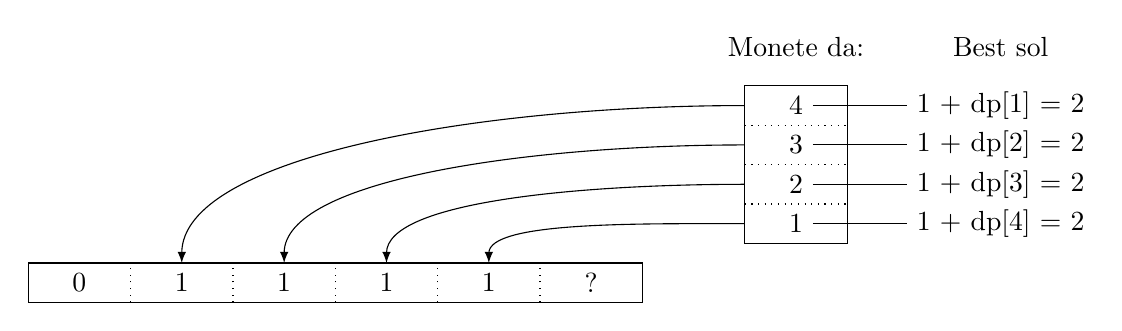
\begin{tikzpicture}[yscale = 0.5, xscale = 1.3]
				            \def\rows{1}
				            \def\columns{6}
				            \newcommand{\shiftx}{0}
				            \newcommand{\shifty}{0}


				            \foreach \x in {0,1,...,\columns}{
						            \draw [dotted](0 + \shiftx,0 + \shifty)++(\x,0)--++(0,\rows);
					            }

				            \foreach \x in {0,1,...,\rows}{
						            \draw (0 + \shiftx,0 + \shifty)++(0,\x)--++(\columns,0);
					            }

				            \draw (\shiftx, \shifty)rectangle++(\columns, \rows);

				            %\draw [-latex](5 - 0.5, 1)to[out=90, in=90](4 - 0.5, 1);
				            \node at (1 - 0.5, \shifty + 0.5) {0};
				            \node at (2 - 0.5, \shifty + 0.5) {1};
				            \node at (3 - 0.5, \shifty + 0.5) {1};
				            \node at (4 - 0.5, \shifty + 0.5) {1};
				            \node at (5 - 0.5, \shifty + 0.5) {1};
				            \node at (6 - 0.5, \shifty + 0.5) {?};

				            \draw (\columns + 1, 1.5)rectangle(\columns + 2, 5.5);

				            \foreach \x in {0,1,...,2}{
						            \draw [dotted](\columns + 1, 2.5 + \x)--++(1,0);
					            }

				            \node (a)at(\columns + 1.5, 2) {1};
				            \node (b)at(\columns + 1.5, 3) {2};
				            \node (c)at(\columns + 1.5, 4) {3};
				            \node (d)at(\columns + 1.5, 5) {4};
				            \node  at(\columns + 1.5, 6.5) {Monete da:};

				            \draw [-latex](\columns + 1, 5)to[out = 180, in=90](1.5, 1);
				            \draw [-latex](\columns + 1, 4)to[out = 180, in=90](2.5, 1);
				            \draw [-latex](\columns + 1, 3)to[out = 180, in=90](3.5, 1);
				            \draw [-latex](\columns + 1, 2)to[out = 180, in=90](4.5, 1);

				            \node (1)at(\columns + 3.5, 2) {1 + dp[4] = 2};
				            \node (2)at(\columns + 3.5, 3) {1 + dp[3] = 2};
				            \node (3)at(\columns + 3.5, 4) {1 + dp[2] = 2};
				            \node (4)at(\columns + 3.5, 5) {1 + dp[1] = 2};
				            \node  at(\columns + 3.5, 6.5) {Best sol};

				            \draw (a)--(1);
				            \draw (b)--(2);
				            \draw (c)--(3);
				            \draw (d)--(4);
			            \end{tikzpicture}

			            La miglior souzione per una somma pari a 5 è quindi 2. Possiamo usare 2 monete in modi diversi ((3,2), (4,1)) per ottenere la somma 5
		            \end{center}
	      \end{itemize}
	\item Mettendo in ordine il concetto intuitivo dobbiamo creare \verb|dp[i]| mettendo nel seguente modo:
	      \begin{itemize}
		      \item Per ogni elemento di \verb|coins| che sia minore di \verb|i| calcolo il numero minimo di monete che è necessario per arrivare ad una somma di \verb|i| utilizzando \verb|dp|. Supponendo di dover includere una moneta di valore \verb|value|, allora il minor numero di monete per arrivare a \verb|i| è dato da
		            \begin{center}
			            \verb|dp[i-value] + 1|
		            \end{center}
		      \item Il valore minimo di monete per arrivare alla somma \verb|i| è il valore minimo fra tutti quelli calcolari al punto precedente
		      \item Occhio ai casi nei quali non è possibile ottenere una somma specifica tramite le monete a disposizione. In questi casi metteremo il valore -1 nel vettore \verb|dp|
	      \end{itemize}
\end{itemize}
\begin{esercizio}{Unique paths \href{https://leetcode.com/problems/unique-paths/description/}{(link)} }
	Un robot si muove su di una griglia {\ttfamily n x m}. Il robot inizialmente è posizionato sulla cella $ \left[0\right]\left[0\right] $ e deve arrivare alla cella $ \left[m-1\right]\left[n-1\right] $. Il robot può muoversi solamente verso il basso e verso destra. Dati due interi {\ttfamily n, m} che indicano la dimensione della griglia, calcolare il numero di percosi possibili
	\vskip3mm
	\vskip3mm
	\underline{Input}
	\vskip3mm
	Gli interi {\ttfamily m} e {\ttfamily n}
	\vskip3mm
	\underline{Output}
	\vskip3mm
	Il numero di percorsi possibili
	\renewcommand{\cellalign}{l}
	\begin{center}
		\begin{tabularx}{\textwidth}{llX}
			\toprule
			Input & Output & Discussione                                                                                        \\
			\midrule
			2 2   & 2      & I percorsi possibili sono $[(R \rightarrow D), (D \rightarrow R)]$                                 \\[12pt]
			3 2   & 3      & I percorsi possibili sono \vskip0mm
			$(R \rightarrow D \rightarrow D)$, $(D \rightarrow D \rightarrow R)$, $\left(D \rightarrow R \rightarrow D\right)]$ \\
			\bottomrule
		\end{tabularx}
	\end{center}
	Complessità ottimale: $ O\left(n \cdot  m\right) $
\end{esercizio}\label{uniquepaths}

L'idea di base è la seguente:
\begin{itemize}
	\item Creo matrice {\ttfamily dp} che salva nella generica cella $ \left[i\right]\left[j\right] $ il numero di percorsi tramite i quali posso arrivare in $ \left[i\right]\left[j\right] $
	\item Inizializzo la prima colonna e la prima riga della matrice a 1: per raggiungere le celle della prima riga e colonna ho un solo modo, ossia rispettivamente spostarmi a destra o spostarmi in basso (non posso tornare indietro)
	\item Per ogni cella che avanza calcolo il valore come la somma della cella a sinistra e della cella a sopra: questo perche per arrivare nella cella $ \left[i\right]\left[j\right] $ posso passare per la cella $ \left[i-1\right]\left[j\right] $ oppure per la cella $ \left[i\right]\left[j-1\right] $. La somma dei modi che ho per arrivare nelle suddette celle è il numero di modi che ho per arrivare nella cella corrente
	\item Una volta generata l'intera tabella, nella ultima cella in basso a destra avro il risultato al problema
\end{itemize}
\begin{gather*}
	\begin{bmatrix}
		1 & 1 & 1 & 1 & 1 & 1 & 1 \\
		1 & 2 & / & / & / & / & / \\
		1 & / & / & / & / & / & / \\
	\end{bmatrix}
	\begin{bmatrix}
		1 & 1 & 1 & 1 & 1 & 1 & 1 \\
		1 & 2 & 3 & / & / & / & / \\
		1 & / & / & / & / & / & / \\
	\end{bmatrix}
	\begin{bmatrix}
		1 & 1 & 1 & 1 & 1 & 1 & 1 \\
		1 & 2 & 3 & 4 & / & / & / \\
		1 & / & / & / & / & / & / \\
	\end{bmatrix}
	\begin{bmatrix}
		1 & 1 & 1 & 1 & 1 & 1 & 1 \\
		1 & 2 & 3 & 4 & 5 & / & / \\
		1 & / & / & / & / & / & / \\
	\end{bmatrix}
	\\
	\begin{bmatrix}
		1 & 1 & 1 & 1 & 1 & 1 & 1 \\
		1 & 2 & 3 & 4 & 5 & 6 & / \\
		1 & / & / & / & / & / & / \\
	\end{bmatrix}
	\begin{bmatrix}
		1 & 1 & 1 & 1 & 1 & 1 & 1 \\
		1 & 2 & 3 & 4 & 5 & 6 & 7 \\
		1 & / & / & / & / & / & / \\
	\end{bmatrix}
	\begin{bmatrix}
		1 & 1 & 1 & 1 & 1 & 1 & 1 \\
		1 & 2 & / & / & / & / & / \\
		1 & 3 & / & / & / & / & / \\
	\end{bmatrix}
	\begin{bmatrix}
		1 & 1 & 1 & 1 & 1 & 1 & 1 \\
		1 & 2 & 3 & / & / & / & / \\
		1 & 3 & 6 & / & / & / & / \\
	\end{bmatrix}
	\\
	\begin{bmatrix}
		1 & 1 & 1 & 1  & 1 & 1 & 1 \\
		1 & 2 & 3 & 4  & / & / & / \\
		1 & 3 & 6 & 10 & / & / & / \\
	\end{bmatrix}
	\begin{bmatrix}
		1 & 1 & 1 & 1  & 1  & 1 & 1 \\
		1 & 2 & 3 & 4  & 5  & / & / \\
		1 & 3 & 6 & 10 & 15 & / & / \\
	\end{bmatrix}
	\\
	\begin{bmatrix}
		1 & 1 & 1 & 1  & 1  & 1  & 1 \\
		1 & 2 & 3 & 4  & 5  & 6  & / \\
		1 & 3 & 6 & 10 & 15 & 21 & / \\
	\end{bmatrix}
	\begin{bmatrix}
		1 & 1 & 1 & 1  & 1  & 1  & 1  \\
		1 & 2 & 3 & 4  & 5  & 6  & 7  \\
		1 & 3 & 6 & 10 & 15 & 21 & 28 \\
	\end{bmatrix}
\end{gather*}


\begin{esercizio}{Unique paths II \href{https://leetcode.com/problems/unique-paths/description/}{(link)} }
	Un robot si muove su di una griglia {\ttfamily n x m}. Il robot inizialmente è posizionato sulla cella $ \left[0\right]\left[0\right] $ e deve arrivare alla cella $ \left[m-1\right]\left[n-1\right] $. Il robot può muoversi solamente verso il basso e verso destra. Sulla griglia possono essere presenti degli ostacoli attraverso i quali il robot non può passare. Data una matrice {\ttfamily obstacles}, nella quale le celle con valore 1 indicano le celle con ostacoli, trovare il numero di percorsi possibili per arrivare nell'ultima cella in fondo a destra
	\vskip3mm
	\vskip3mm
	\underline{Input}
	\vskip3mm
	Gli interi {\ttfamily m} e {\ttfamily n} e nelle {\ttfamily m} righe successiva gli elementi della matrice {\ttfamily obstacles}
	\vskip3mm
	\underline{Output}
	\vskip3mm
	Il numero di percorsi possibili
	\renewcommand{\cellalign}{l}
	\begin{center}
		\begin{tabularx}{\textwidth}{llX}
			\toprule
			Input & Output & Discussione                                                                     \\
			\midrule
			\makecell{3 3                                                                                    \\ 0 0 0 \\ 0 1 0 \\ 0 0 0}& 2  & I percorsi possibili sono \vskip0mm
			$[(R \rightarrow R \rightarrow D \rightarrow D), (D \rightarrow D \rightarrow R \rightarrow R)]$ \\
			\bottomrule
		\end{tabularx}
	\end{center}
	Complessità ottimale: $ O\left(n \cdot  m\right) $
\end{esercizio}

L'idea è molto simile al problema \hyperref[uniquepaths]{Unique paths}, con l'unica differenza che dobbiamo tenere in considerazione i casi in cui una rotta è preclusa da un ostacolo. Inoltre, anzichè creare una nuova matrice {\ttfamily dp}, possiamo usare direttamente la matrice {\ttfamily obstacles} che ci viene data.
\begin{itemize}
	\item Riempio la prima colonna e riga della matrice {\ttfamily obstacles} con valore 1 fino al primo ostacolo. Dal primo ostacolo in poi avrò solo celle irraggiungibili. Setto le celle irraggiungibili con valore -1, in quanto usando 1 rischierei di confondere le celle irraggiungibili con le celle raggiungibili da 1 solo cammino
	\item Calcolo le celle rimanenti con la stessa logica usata in \hyperref[uniquepaths]{Unique paths}, tenendo conto però che:
	      \begin{itemize}
		      \item Nel caso ci sia un ostacolo nella cella a sinistra o in alto a quella corrente non posso arrivare da quella direzione. Se non rimane nemmeno una rotta possibile posso impostare il valore della della a -1, in quanto non riesco a ragiungerla in nessun modo
		      \item Nel caso ci sia un ostacolo nella cella corrente ({\ttfamily obstacles[i][j] == 1}) cambio il valore e metto -1, onde evitare ambiguità come spiegato precedentemente
	      \end{itemize}
	\item Ancora una volta, nella cella $ \left[m-1,n-1\right] $ ci sarà la soluzione del problema
\end{itemize}

\begin{gather*}
	\begin{bmatrix}
		0 & 0 & 0 \\
		0 & 1 & 0 \\
		0 & 0 & 0 \\
	\end{bmatrix}
	\xrightarrow{\text{riempio prima riga e colonna}}
	\begin{bmatrix}
		1 & 1 & 1 \\
		1 & 1 & 0 \\
		1 & 0 & 0 \\
	\end{bmatrix}
	\xrightarrow{\text{ cambio ostacolo in -1}}
	\begin{bmatrix}
		1 & 1  & 1 \\
		1 & -1 & 0 \\
		1 & 0  & 0 \\
	\end{bmatrix}
	\\
	\begin{bmatrix}
		1 & 1  & 1 \\
		1 & -1 & 1 \\
		1 & 0  & 0 \\
	\end{bmatrix}
	\begin{bmatrix}
		1 & 1  & 1 \\
		1 & -1 & 0 \\
		1 & 1  & 0 \\
	\end{bmatrix}
	\begin{bmatrix}
		1 & 1  & 1 \\
		1 & -1 & 1 \\
		1 & 1  & 2 \\
	\end{bmatrix}
\end{gather*}
\section{Ripassone}
\subsection{Classi}
\begin{itemize}
	\item Una classe è un insieme di \underline{metodi} (funzioni) e \underline{attributi} (variabili).
	\item La classe definisce \underline{il modello} e la struttura del dato che vogliamo rappresentare. Il dato effettivo si chiama \underline{oggetto} o \underline{istanza}
	\item Quando creaiamo una classe viene chiamato il \underline{costruttore}
	      \begin{itemize}
		      \item Il costruttore ha forma : \verb|public nomeClasse(...){...}|
		      \item Si può fare qualunque cosa nel costruttore ma di solito si inizializzano gli attributi della classe
		      \item Se non viene definito esplicitamente, allora le il compilatore ne inserisce uno che non fa nulla
	      \end{itemize}
\end{itemize}

\subsection{Ereditarietà}
L'ereditarietà è un meccanismo che permette di, per l'appunto, ereditare il codice di una classe all'interno di un'altra.
\begin{itemize}
	\item Si effettua utilizzando la keyword \verb|extend|
	\item Se \verb|B extend A|, allora \verb|B| possiede tutti gli attributi ed i metodi di \verb|A|
\end{itemize}
\subsubsection{Keyword super}
La keyword \verb|super| può essere usata in una classe che estende un'altra in due modi:
\begin{itemize}
	\item \verb|super(arg1, arg2...)| chiama il costruttore della super classe
	\item \verb|super.method(arg1, arg2...)| il metodo indicato della super classe
\end{itemize}
\subsubsection{Principio di sostituzione di Liskov}
\textit{Se} \verb|B extend A|, \textit{allora in un programma ben scritto posso sosituire ogni istanza di} \verb|A| \textit{con una di} \verb|B|\textit{, ottenendo lo stesso comportamento}
\subsection{Classi e metodi astratti}
Una classe astratta è una classe che \underline{non può essere istanziata}. Questo serve quando dal punto di vista logico una classe deve per forza essere una delle sue sottoclassi. Ad esempio nella seguente gerarchia:
\begin{center}
	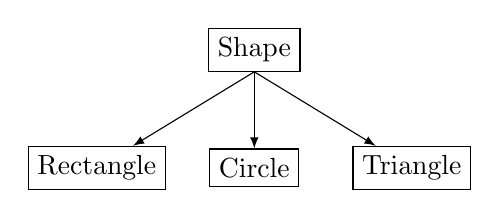
\begin{tikzpicture}
		\node [draw](a)at (0,0)  {Shape};
		\node [draw](1)at (-2,-1.5)  {Rectangle};
		\node [draw](2)at (0,-1.5)  {Circle};
		\node [draw](3)at (2,-1.5)  {Triangle};
		\draw [-latex](a.south)--(1);
		\draw [-latex](a.south)--(2);
		\draw [-latex](a.south)--(3);
	\end{tikzpicture}
\end{center}
Ha senso istanziare un oggetto di tipo \verb|Shape|?
\vskip3mm
Una classe astratta può contenere \underline{metodi astratti}, ossia metodi che non abbiano un corpo. Questi servono per far si che la loro implementazione sia \underline{obbligatoria} per ognuna della sottoclassi

\subsection{Override e overloading}
\begin{itemize}
	\item \textbf{Override:} ridefinisco una funzione con \underline{stesso nome, argomenti e valore di ritorno} in una sottoclasse
	\item \textbf{Overload:} definisco una funzione che abbia \underline{lo stesso nome} ma \textit{parametri e valore di ritorno diversi} nella stessa classe o in una classe che estende
\end{itemize}

Ad esempio, supponiamo di avere due classi \verb|A| e \verb|B| e \verb|B extend A|
\begin{center}
	\ttfamily
	\begin{tabular}{|l|l|}
		\hline
		A            & B            \\
		\hline
		f1()         & f1(int a)    \\
		f1(String s) & f1(float a)  \\
		\hline
		f2()         & f2()         \\
		f2(String s) & f2(String s) \\
		\hline
	\end{tabular}
\end{center}
Quando si fa overload, il valore di ritorno \underline{non} può essere l'unica differenza nella \footnote{Con signature si intende l'insieme di nome di una funzione, tipo e numero dei suoi argomenti}{signature} delle due funzioni.

\subsection{Tipo statico e dinamico}
Il tipo statico decreta:
\begin{itemize}
	\item Quali funzioni posso chiamare tramite un'istanza
	\item Quale versione dell'override è chiamata
\end{itemize}
Il cast modifica il \underline{tipo statico}. Il tipo dinamico decreta invece:
\begin{itemize}
	\item Quale versione dell'override viene chiamata
	\item Risultato operatore instanceof
\end{itemize}
Quindi a tutti gli effetti, il tipo dinamico indica la "conformazione" della zona di memoria indicata da una variabile
\subsubsection{instanceof}
\verb|instanceof| è un operatore che ritorna true se il tipo dinamico della prima variabile estende quello della seconda:
\begin{center}
	\verb|variabile instanceof Tipo|
\end{center}
Ritorna \verb|true| se \verb|Type(variabile) extends Tipo|

\subsection{Cast}
Il cast è un meccanismo per cambiare il \underline{tipo statico} di una istanza di una classe. Si effettua mettendo davanti ad una variabile il tipo a cui vogliamo castare fra parentesi tonde: \verb|(Tipo)variabile|. Supponendo di avere \verb|B extends A|
\begin{itemize}
	\item \verb|downcast| (\verb|(B)A|) permette di "convertire" una classe in una sottoclasse. \verb|A -> B|. Può fallire a \textit{runtime} se il tipo dinamico di \verb|A| è più in basso nella gerarchia delle classi rispetto a \verb|B|
	\item \verb|upcast| permette di "convertire" una classe nella sua superclasse. Non può fallire a patto che \verb|A| appartenga alla stessa gerarchia
\end{itemize}

\subsection{Late binding}
Il late binding è il meccanismo per cui, nel momento in cui chiamo un metodo su di una istanza di tipo statico \verb|A| e tipo dinamico \verb|B|, l'override della funzione chiamata è quella definita in \footnote{In realtà, viene chiamato l'override presente nella "versione più recente", ossia quella che si trova più il basso nella gerarchia delle classi}{\verb|B|}
\begin{tikzpicture}

\end{tikzpicture}
\end{document}
